\documentclass[10pt]{article}

%Packages with options
\usepackage[english]{babel}
\usepackage[mathscr]{euscript}
\usepackage[margin = 1in]{geometry}
\usepackage[utf8]{inputenc}
\usepackage[small]{titlesec}

% Primary Packages
\usepackage{adjustbox}
\usepackage{amsmath}
\usepackage{amssymb}
\usepackage{amsthm}
\usepackage{bm}
\usepackage{commath}
\usepackage{chngcntr}
\usepackage{dsfont}
\usepackage{econometrics}
\usepackage{fancyhdr}
\usepackage{gensymb}
\usepackage{graphicx}
\usepackage{hyperref}
\usepackage{longtable}
\usepackage{marginnote}
\usepackage{mathtools}
\usepackage{natbib}
\usepackage{mdframed}
\usepackage{parskip}
\usepackage{setspace}
\usepackage{subfigure}
\usepackage{tabularx}
\usepackage{textcomp}

% Secondary Pacakges [need to be loaded later]
\usepackage{breqn}

% Setting up page style 
\pagestyle{fancy}
\setlength{\headheight}{23pt}
\renewcommand{\headrulewidth}{0pt}
\renewcommand{\sectionmark}[1]{%
\markboth{\thesection\quad #1}{}}
\fancyhead{}
\fancyhead[R]{\leftmark}
\fancyfoot{}
\fancyfoot[C]{\thepage}
\linespread{1}

% Change expectation and probability to doublescript
\renewcommand{\E}{\mathbb{E}}
\renewcommand{\P}{\mathbb{P}}

% Declare a shortcut for \theta and \Theta
\renewcommand{\t}{\theta}
\newcommand{\T}{\Theta}

% Make capital vectors commands from econometrics packages
\newcommand{\vA}{\mathbf{A}}
\newcommand{\vB}{\mathbf{B}}
\newcommand{\vC}{\mathbf{C}}
\newcommand{\vD}{\mathbf{D}}
\newcommand{\vE}{\mathbf{E}}
\newcommand{\vF}{\mathbf{F}}
\newcommand{\vG}{\mathbf{G}}
\newcommand{\vH}{\mathbf{H}}
\newcommand{\vI}{\mathbf{I}}
\newcommand{\vJ}{\mathbf{J}}
\newcommand{\vK}{\mathbf{K}}
\newcommand{\vL}{\mathbf{L}}
\newcommand{\vM}{\mathbf{M}}
\newcommand{\vN}{\mathbf{N}}
\newcommand{\vO}{\mathbf{O}}
\newcommand{\vP}{\mathbf{P}}
\newcommand{\vQ}{\mathbf{Q}}
\newcommand{\vR}{\mathbf{R}}
\newcommand{\vS}{\mathbf{S}}
\newcommand{\vT}{\mathbf{T}}
\newcommand{\vU}{\mathbf{U}}
\newcommand{\vV}{\mathbf{V}}
\newcommand{\vW}{\mathbf{W}}
\newcommand{\vX}{\mathbf{X}}
\newcommand{\vY}{\mathbf{Y}}
\newcommand{\vZ}{\mathbf{Z}}

% Declare some shortcuts
\newcommand{\andbox}{\hbox{ }\text{ and }\hbox{ }}
\newcommand{\DeltaT}{\tilde{\Delta}}
\newcommand{\ind}{\mathds{1}}
\newcommand{\muH}{\hat{\mu}}
\newcommand{\nuH}{\hat{\nu}}
\newcommand{\nuT}{\tilde{\nu}}
\newcommand{\PK}{(K)}
\newcommand{\ris}{\rho_{i}^*}
\newcommand{\sigmaH}{\hat{\sigma}}
\newcommand{\thetaH}{\hat{\theta}}
\newcommand{\thetaT}{\tilde{\theta}}
\newcommand{\wcov}{\rightsquigarrow}


% Declare New Math Operators
\DeclareMathOperator{\argmax}{arg\,max}
\DeclareMathOperator{\argmin}{arg\,min}
\DeclareMathOperator{\cube}{Cub}
\DeclareMathOperator{\do}{do}
\DeclareMathOperator{\err}{err}
\DeclareMathOperator{\id}{id}
\DeclareMathOperator{\Poisson}{Poisson}
\DeclareMathOperator{\polylog}{polylog}
\DeclareMathOperator{\supp}{supp}
\DeclareMathOperator{\sign}{sign}
\DeclareMathOperator{\Var}{Var}


% Useful numberthis tag
\newcommand\numberthis{\addtocounter{equation}{1}\tag{\theequation}}

% Define Theorems, Definitions, Corollarys, etc.
\newtheoremstyle{exampstyle}
  {1em plus .2em minus .1em}%   Space above
  {1em plus .2em minus .1em}%   Space below
  {} % Body font
  {} % Indent amount
  {\bfseries} % Theorem head font
  {.} % Punctuation after theorem head
  {.5em} % Space after theorem head
  {} % Theorem head spec (can be left empty, meaning `normal')


 {
    \theoremstyle{exampstyle}

    \newtheorem{assumption}{Assumption}
    \newtheorem*{assumption*}{Assumption}
    \newtheorem{definition}{Definition}
    \newtheorem*{definition*}{Definition}    
    \newtheorem{example}{Example}
    \newtheorem*{example*}{Example}
    \newtheorem{remark}{Remark}
    \newtheorem*{remark*}{Remark}
    \newtheorem{specification}{Specification}
    \newtheorem*{specification*}{Specification}
 }

\newtheorem{corollary}{Corollary}
\newtheorem*{corollary*}{Corollary}
\newtheorem{lemma}{Lemma}
\newtheorem*{lemma*}{Lemma}
\newtheorem{prop}{Proposition}
\newtheorem*{prop*}{Proposition}
\newtheorem{theorem}{Theorem}
\newtheorem*{theorem*}{Theorem}

%Define command for blocked theorems
\newcommand{\blocktheorem}[1]{%
  \csletcs{old#1}{#1}% Store \begin
  \csletcs{endold#1}{end#1}% Store \end
  \RenewDocumentEnvironment{#1}{o}
    {\par\addvspace{1.5ex}
     \noindent\begin{minipage}{\textwidth}
     \IfNoValueTF{##1}
       {\csuse{old#1}}
       {\csuse{old#1}[##1]}}
    {\csuse{endold#1}
     \end{minipage}
     \par\addvspace{1.5ex}}
}
\blocktheorem{assumption}
\blocktheorem{definition}
\blocktheorem{theorem}
\blocktheorem{prop}
\blocktheorem{specification}
\raggedbottom

%Reset equation counters for each section
\counterwithin*{assumption}{section}
\counterwithin*{corollary}{section}
\counterwithin*{definition}{section}
\counterwithin*{equation}{section}
\counterwithin*{figure}{section}
\counterwithin*{footnote}{subsection}
\counterwithin*{lemma}{section}
\counterwithin*{prop}{section}
\counterwithin*{remark}{section}
\counterwithin*{specification}{section}
\counterwithin*{table}{section}
\counterwithin*{theorem}{section}

% Set bibliography style
\bibliographystyle{apalike}

% Title, Author, Date
\title{Readings on Moment Inequality Methods}
\author{Manu Navjeevan}
\date{\today}

%%%%%%%%%%%%%%%%%%%%%%%%%%%%%%%%%%%%%%%%%%%%%%%%%%%%
%MAIN DOCUMENT
%%%%%%%%%%%%%%%%%%%%%%%%%%%%%%%%%%%%%%%%%%%%%%%%%%%%

\begin{document}

% Title Page and Table of Contents
\maketitle  
\tableofcontents
\newpage

% Covered Papers
%!TEX root = /Users/manunavjeevan/Desktop/Research/Moment Inequality Methods/Annotated Literature Review/inequalityLitReview.tex

\section{A Practical Method for Testing Many Moment Inequalities; \textit{\small Yuehao Bai, Andres Santos, Azeem M. Shaikh}}

\subsection{Introduction}

Setup: $\{X_i\}_{i=1}^n$ i.i.d with distribution $P\in P_n$ on $R^{\mathscr{p}_n}$. Consider the problem of testing 

\begin{equation}
\label{eq:hypothesisTest}
	H_0: P\in \mathbf{P}_{0,n}\hbox{ }\text{ versus }\hbox{ }H_1: P\in \mathbf{P}_{1,n}
\end{equation}
where
\begin{equation}
\label{eq:restrictedSet}
	\mathbf{P}_{0,n} \equiv \{P\in \mathbf{P}_n: E_P[X_i]\leq 0\}
\end{equation}
and $\mathbf{P}_{1,n} = \mathbf{P}_n/\mathbf{P}_{0,n}$. The inequality in \ref{eq:restrictedSet} is interpreted component wise and $\mathbf{P}_n$ is a large class of possible distributions for the observed data. Indexing both the number of moments $p_n$ and the class of possible distributions by the sample size allows for the number of moments to grow (rapidly) with the sample size $n$. Goal is to construct test that are uniformply consistent in level; i.e
\begin{equation}
	\label{eq:uniformConsistency}
	\lim\sup_{n\rightarrow \infty} \sup_{P\in\mathbf{P}_{0,n}} E_P[\phi_n] \leq \alpha
\end{equation}
A test can be viewed as a function of the data $\phi_n = \phi_n: \mathscr{X}^n \rightarrow \{0,1\}$ where $\mathscr{X}^n$ is generally some subset of $\mathbb{R}^n$ where the data takes its values. 

There are a large class of problems in economics in which the number of moments is large. For example, in the entry models as in Cilberto and Tamer (2009) the number of moment inequalities to check is $p_n = o(2^{m+1})$ where $m$ is the number of firms. Apart from Chernozukhov et. al (2019), this has typically been done by limiting $\mathbf{P}_n$ so that the number of moments $p_n$ are small. Canay and Shaikh (2017) provide a detailed review of these tests. This paper focuses on the two step testing procedure of Romano et. al (2014). Test is shown to satisy (\ref{eq:uniformConsistency}) under assumptions on $\mathbf{P}_n$ that restrict $p_n$ to not depend on $n$. However, the test is ``practical'' in that it is computationally feasible even if the number of moments is large. \textbf{Paper shows that the test of Romano et. al (2014) continues to satisy (\ref{eq:uniformConsistency}) for a large class of distributions that permits the number of moments $p_n$ to grow exponentially with the sample size $n$.}

Theoretical analysis relies on Chernozhukov et. al (2013, 2017) on the high dimensional CLT. This is seminal work. Allen (2018) argues that the test proposed Romano et al. (2014) is more powerful in finite samples then the test proposed by Chernozhukov et al. (2019). 

\subsection{Main Result}

Begin this section by describing the testing procedure in Romano et al. (2014). To do so, best to introduce some further notation. For $1\leq j\leq p_n$ let $X_{i,j}$ denote the $j$th component of $X_i$ and set 
\begin{align}
    \bar{X}_{j,n} &\equiv \frac{1}{n}\sum_{i=1}n X_{i,j} \label{eq:XjBar} \\
    S_{j,n}^2 &\equiv \frac{1}{n}\sum_{i=1}^n (X_{i,j} - \bar{X}_{j,n})^2 \label{eq:Sj2}
\end{align}
Can also use the notation $\mu_j(p) \equiv E_P[X_{i,j}]$ and $\sigma_j^2(P)\equiv \Var_{P}[X_i,j]$ so that (\ref{eq:XjBar}) and (\ref{eq:Sj2}) can be expressed as $\mu_j(\hat{P}_n)$ and $\sigma_j^2(\hat{P}_n)$, respectively, where $\hat{P}_n$ is the empirical distribution of $\{X_i\}_{i=1}^n$. Focus on a test that rejects for large values of 
\[T_n \equiv \max\left\{ \max_{1\leq j \leq p_n}\frac{\sqrt{n}\bar{X}_{j,n}}{S_{j,n}} ,0\right\}\] 
In defining critical value, useful to introduce an i.i.d sequence of random variables with distribution $\hat{P}_n$ conditional on $\{X_i\}_{i=1}^n$, which we will denote $X_i^*, i = 1, \dots, n$. Further define $\bar{X}_{j,n}^*$ and $(S_{j,n}^*)^2$ analagously to before, but substituting in $X_i^*$. Critical value for $T_n$ is given by 
\begin{equation}
	\label{eq:critVal}
	\hat{c}_n^{(2)}(1 - \alpha + \beta) \equiv \inf \mathscr{S}_n(1-\alpha +\beta)
\end{equation}
where 
\[\mathscr{S}_n(a) \equiv \left\{c\in \mathbb{R}: \mathbb{P}\left[\max\left\{ \max_j \frac{\sqrt{n}(\bar{X}_{j,n}^* - \bar{X}_{j,n} + \hat{\mu}_{j,n})}{S_{j,n}^*},0 \right\} \leq c \hbox{ }\bigg|\hbox{ } \{X_i\}_{i=1}^n\right] \geq a \right\}\]
Here $\alpha \in (0,0.5)$ is the nominal level of the test and $\beta \in (0,\alpha)$ and 
\begin{equation}
	\label{eq:muHat}
	\hat{\mu}_{j,n} \equiv \min\left\{\bar{X}_{j,n} + \frac{S_{j,n}}{\sqrt{n}} \hat{c}_n^{(1)}(1-\beta), 0\right\}
\end{equation}
with 
\[\hat{c}_n^{(1)} \equiv \inf\left\{ c \in \mathbb{R}: \mathbb{P}\left[\max_{1\leq j\leq p_n} \frac{\sqrt{n}(\bar{X}_{j,n} - \bar{X}_{j,n}^*)}{S_{j,n}^*} \leq c \hbox{ }\bigg|\hbox{ }  \{X_i\}_{i=1}^n \right] \geq 1- \beta \right\}\]
The test is then
\begin{equation}
	\label{eq:testRSW}
	\phi_n^{\text{RSW}} \equiv \mathds{1}\left\{T_n \geq \hat{c}_n^{(2)}(1-\alpha+\beta)\right\}
\end{equation}
Motivating this choice of critical value it is useful to note that the test statistic $T_n$ satisfies
\begin{equation}
	\label{eq:decomp}
	T_n = \max\left\{\max_j \left(\frac{\sqrt{n}(\bar{X}_{j,n} - \mu_j(P))}{S_{j,n}} + \frac{\sqrt{n}\mu_{j}(P)}{S_{j,n}} \right), 0 \right\}
\end{equation}
Decomposition highlights that the main impedment in approximating the distribution of $T_n$ is the presence of nuisance parameters $\sqrt{n}\mu_j(P)$ for $1\leq j \leq p_n$.\footnote{I'm not entirely sure why they cannot be consistently estimated. I think this is because we are only partially identified.} Though these nuisance parameters cannot be consistently estimated, Romano et al (2014) observe that it may still be possible to construct a suitably valid confidence region for them. 

Lemma in Appendix employs Romano insight and high dimensional CLT of Chernozhukov et al. (2017) to show that, under conditions that permit $p_n$ to grow rapidly with the sample size $n$, $\sqrt{n}\mu_j(P) \leq \sqrt{n}\hat{\mu}_{j,n}$ for all $j \leq p_n$ with pr. approximately no less than $1-\beta$ whenever the null hypothesis in (\ref{eq:hypothesisTest}) is true. Since $T_n$ is monotonically increasing in the nuisance parameters $\sqrt{n}\mu_j(P)$ for all $1\leq j \leq p_n$ it follows that, viewed as a funtion of these nuisance parameters, any quantile of $T_n$ is maximized over said confidence region by setting $\sqrt{n}\mu_j(P) = \sqrt{n}\hat{\mu}_{j,n}$ for all $j$. Then, the critical value $\hat{c}_n^{(2)}(1-\alpha + \beta)$ is a bootstrap estimate of the $1-\alpha + \beta$ quantile of $T_n$ under the ``least favorable'' nuisance parameter value $\sqrt{n}\mu_j(P) = \sqrt{n}\hat{\mu}_{j,n}$ for all $j$. The $1-\alpha-\beta$ quantile is employed instead of $\beta$ to account for that, with pr. appx no greater than $\beta$, $\sqrt{n}\mu_j(P)>\sqrt{n}\hat{\mu}_{j,n}$. Analysis of test (\ref{eq:testRSW}) hinges on following assumption:

\begin{assumption} 
\label{eq:assumption2.1}
Assume (i) $\{X_i\}_{i=1}^n$ is an i.i.d sample with $X_i \in \mathbb{R}^{p_n}$ and $X_i \sim P \in \mathbf{P}_n$; (ii) $\sigma_j(P) > 0$ for all $1 \leq j \leq p_n$ and $P \in \mathbb{P}_n$; (iii) For $k = 1,2$, there is a $M_{k,n} < \infty$ such that $E_P[|X_{i,j} - \mu_j(P)|^{2+k}] \leq \sigma_j^{2+k}(P)M_{k,n}^k$ for all $1\leq j \leq p_n$ and $P\in \mathbf{P}_n$; (iv) There exists a $B_n < \infty$ such that $E_P\left[\max_{1\leq j \leq p_n}\left|X_{i,j} -\mu_j(P)\right|^4\right] \leq B_n^4$ for all $P\in \mathbf{P}_n$; (v) $(M_{1,n}^2 \vee M_{2,n}^2 \vee B_n^2)\log^{3.5}(p_n n) = o(n^{(1-\delta)/2})$ for some $\delta \in (0,1)$
\end{assumption}

\ref{eq:assumption2.1}(i) formalizes that $\{X_i\}_{i=1}^n$ be an i.i.d sample, while Assumption \ref{eq:assumption2.1}(ii) requires the variance of $X_{i,j}$ to be positive for all $P \in \mathbb{P}_n$ and $1 \leq j \leq p_n$.\ref{eq:assumption2.1}(iii) imposes a uniform in $P$ and $j$ bound on the standardized moments of $X_{i,j}$. Condition is a strengthening of the uniform integrability requirements of Romano et al (2014) required so study a setting in which $p_n$ diverges to infinity. Part (iv) bounds the 4th moments of the maximim of $X_{i,j}$. Finally, (v) states the main conditiion governing how fast $p_n$ can grow with $n$. Under suitable moment restrictions on $X_{i,j}$, $p_n$ may grow exponentially with $n$. Now ready for main result

\begin{theorem}
	If Assumption \ref{eq:assumption2.1} holds, $\alpha \in (0,\frac{1}{2})$ and $0 < \beta < \alpha$, then $\phi_n^{\text{RSW}}$ as defined in (\ref{eq:testRSW}) satisfies uniform consistency in level as defined in (\ref{eq:uniformConsistency})
\end{theorem}

The rest of this paper goes through some simulations. It is also just a working paper at the moment. Probably it is best to go through the main proof; but I will print it out and make some notes on this. 


%!TEX root = /Users/manunavjeevan/Desktop/Research/Moment Inequality Methods/Annotated Literature Review/inequalityLitReview.tex

\section{Inference on Causal and Structural Parameters Using Many Moment Inequalities; \textit{\small Victor Chernozhukov, Denis Chetverikov, and Kengo Kato (ReStud, 2019)}}\label{sec:CCK-2019}

\subsection{Introduction}

In recent years, moment inequalities framework has developed into a powerful tool for inference on causal and structural parameters in partially identified models. Many papers study models with a finite and fixed number of conditional and unconditional moment inequalities. IN practice the number of moment inequalities implied by the model is often large. 

Examples of testing (very) many moment inequalities
\begin{itemize}
	\item Consumer is selecting a bundle of products for purchase and moment inequalities come from revealed preference argument (Pakes, 2010)
	\item Market structure model of Ciliberto and Tamer (2009), number of moment inequalities equals the number of possible combinations of firms that could potentially enter the market (grows exponentially in the number of firms)
	\item Dynamic model of imperfect competition of Bajari, Benkard, Levin (2007)m where deviations from optimal policy serve to define many moment inequalities
	\item Beresteanu, Molchanov, Molinari (2011), Galichon and Henry (2011)\footnote{This seems like a good place to start reading}, Chesher, Rosen, Smolinksi (2013), and Chester and Rosen (2013)
\end{itemize}
Many examples have inportant in that the many inequalities under consideration are ``unstructured'', they cannot be viewed as unconditional moment inequalities generated froma small number of conditional inequalities with a low-dimensional conditioning variable. So existing inference methods for conditional moment inequalities, though fruitful in many cases 

Formally describing the problem, let $\{X_i\}_{i=1}^n$ be a sequence of i.i.d random vectors in $\mathbb{R}^p$, where $X_i = (X_{i1},\dots,X_{ip})^T$, with a common distribution denoted by $\mathscr{L}_X$. For $j \leq p$, we write $\mu_j := \mathbb{E}[X_{1j}]$. Interested in testing the null hypothesis 
\begin{equation}
	\label{eq:CCK-1}
	H_0 :\mu_j \leq 0\hbox{ }\text{ for all }j = 1,\dots,p
\end{equation}
Against the alternative 
\begin{equation}
	\label{eq:CCK-2}
	H_1: \mu_j > 0 \hbox{ }\text{ for some }j = 1,\dots,p
\end{equation}
Refer to (\ref{eq:CCK-1}) as the moment inequalities and say the $j$th moment is satisfied (viloated) if $\mu_j \leq 0$ ($\mu_j > 0$). Paper will allow number of moment inequalities $p \gg n$. Consider a test statistic given by the maximum over $p$ Studentized (t-type) inequality specific statistic. Consider critical values based upon (i) the union bound combined with a moderate deviation inequality for self-normalized sums and (ii) bootstrap methods. Among bootstrap methods, consider multiplier and emppirical bootstrap methods. These are simulation based and computationally more difficult, but take into account correlation structure and yeild lower critical values. SN method is particularly useful for grid search when the researcher is interested in constricting a confidence interval for identified set. 

Also consider two-step methods incorporating inequality selection procedutes. Two-step methods get rid of most uninformative inequalities, that is inequalities with $\mu_j < 0$ if $\mu_j$ is not too close to 0. Also develop novel three-step methods by incorporating double inequality selection procedures. These are suitable in parametric modesl defined via momoent inequalities and allow to drop weakly informative inequalities in addition to uninformative inequalities.\footnote{Can be extended to nonparametric models as well}. Results can be used for construction of confidence regions for identifiable parameters in partially identified models defined by moment inequalities. Show that results are asymptotically honest (don't quite know what this means).

Literature testing unconditional moment inequalities is large. See White (2000), Chernozhukov, Hong, and Tamer (2007), Romano and Shaikh (2008), Rosen (2008), Andrews and Guggenberger (2009), Andrews and Soares (2010), Canay (2010), Bugni (2011), Andrews and Jia-Barwick (2012), and Romano, Shaikh, and Wolf (2014). 

In this paper we implicitly assume that $X_1, \dots, X_n$ and $p$ are indexed by $n$. Mainly interested in the case that $p = p_n \rightarrow \infty$ as $n \rightarrow \infty$

\subsection{Motivating Examples}

Section provides examples that motivate the framework where the number of moment inequalities $p$ is large and potentially much larger than the sample size $n$. In these examples, one actually has many conditional rather than unconditional inequalities. Results cover conditioning as well. 

\subsubsection{Market Structure Model}

Let $m$ denote the number of firms that could potentially enter the market. Let $m$-tuple $D = (D_1, \dots, D_m)$ denote entry decisions of these firms. That is, $D_j = 1$ if the firm $j$ enters the market and $D_j = 0$ otherwise. Let $\mathscr{D}$ denote the possible values of $D$. We have that $|\mathscr{D}| = 2^m$. 

Let $X$ and $\epsilon$ denote the (exogeneous) characteristics of the market as well as characteristics of the firms that are observed and not observed by the researcher, respectively. The profit of the firm $j$ is given by 
$$\pi_j(D, X, \epsilon, \theta)$$
where $\pi_j$ is known up to a parameter $\theta$. Both $X$ and $\epsilon$ are observed by the firms and a Nash Equilibrium is played so that, for each $j$,
$$\pi_j((D_j, D_{-j}),X, \epsilon, \theta) \geq \pi_j((1-D_j, D_{-j}), X, \epsilon, \theta)$$
$D_{-j}$ denotes the decisions of all firms excluding the firm $j$. Then one can find set-valued functions $R_1(d, X, \theta)$ and $R_2(d, X, \theta)$ such that $d$ is the unique equilibrium whenever $\epsilon \in D_1(d,X, \theta)$ and $d$ is \textit{an} equilibrium whenever $\epsilon \in R_2(d,X, \theta)$. In the second case, the probability that the researcher sees $d$ as an equilibrium depends on the equilibrium selection mechanism. Without further information, anything can be in $[0,1]$. Therefore we have the following bounds 
\begin{align*}
	\mathbb{E}[\mathds{1}\{\epsilon \in R_1(d,X, \theta\}|X] &\leq \mathbb{E}[{\mathds{1}\{D=d\}|X}] \\
	&\leq \mathbb{E}[\mathds{1}\{\epsilon \in R_1(d,X,\theta) \cup R_2(d,X,\theta) \} | X]
\end{align*}
Further assuming that the conditional distribution of $\epsilon$ given $X$ is known (or known up to a parameter that is part of $\theta$), both the LHS and RHS of these inequalites can be calculated. Denote them $P_1(d, X, \theta)$ and $P_2(d,X,\theta)$, respectively to obtain 
\begin{equation}
	\label{2:CilbertoTamerInequalities}
	P_1(d, X, \theta) \leq \mathbb{E}[\mathds{1}\{D=d\}|X] \leq P_2(d,X,\theta)
\end{equation}
for all $d \in \mathds{D}$. These can be used for inference on the parameter $\theta$. Note that the number of inequalities in (\ref{2:CilbertoTamerInequalities}) is $2|\mathscr{D}| = 2^{m+1}$. This is a large number, even if $m$ is moderately large. Moreover, these inequalities are conditional on $X$. So, they can be transformed into a large and increasing number of unconditional moment inequalities as described above. Also, if the firms have more than two decisions, the number of inequalities will be even larger. 

Some other examples are given, but I won't cover them in notes. 

\subsection{Test Statistic}

Begin preparing some notation. Assume that 
\begin{equation}
	\label{eq:CCK-12}
	\mathbb{E}[X_{1,j}^2] < \infty, \sigma_j^2 := \Var(X_{1,j}) > 0, j = 1,\dots, p
\end{equation}
For $j = 1,\dots,p$ let $\muH_j$ and $\sigmaH_j$ be the sample mean and variance of $\{X_{i,j}\}_{i=1}^n$. Many different possible test statistics. Somewhat natural to consider statistics that take large values thehn some of $\hat{\mu}_j$'s are large. In this paper focus on statistic that takes large values when at least one of $\muH_j$ are large. 

In specific, focus on the following test statistic:
\begin{equation}
	\label{2:testStat}
	T = \max_{1\leq j \leq p}\frac{\sqrt{n}\muH_j}{\sigmaH_j}
\end{equation}
Large values of $T$ indicate a likely violation of $H_0$, so it is natural to consider tests of the form 
\[T > c \implies \text{ reject } H_0\]
where $c$ is appropriately chosen so that the test approximately has size $\alpha \in (0,1)$. Consider various ways for calculating critical values and prove their validity. 

\subsection{Critical Values}

Now move to define critical values for $T$ such that under $H_0$, the probability of rejecting $H_0$ does not exceed size $\alpha$ asymptotically. Methods are ordered bu increasing computational complexity, increasing strength of required conditions, and also increasing power. Basic idea for the construction of critical values for $T$ lies in the fact, that, under $H_0$:
\[T \leq \max_{1\leq j \leq p} \frac{\sqrt{n}(\muH_j - \mu_j)}{\sigmaH_j} \]
Consider two approaches to constructing such critical values: self-normalized and bootstrap methods. Also consider two- and three-step variants of the methods by incorporating inequality selection. 

Following notation used:
\[Z_{ij} = (X_{ij} - \mu_j)/\sigma_j\hbox{ }\text{ and }\hbox{ }Z_i = (Z_{i1}, \dots, Z_{ip})^T \]
Observe that $\mathbb{E}[Z_{ij}] = 0$ and $\mathbb{E}[Z_{ij}^2] = 1$. Define 
\[M_{n,k} = \max_{1\leq j \leq p}\left( \mathbb{E}\left[|Z_{1,j}|^k\right]   \right)^{1/k},k = 3,4,\hbox{ }\text{ and }B_n = \left(\mathbb{E}\left[\max_{1\leq j \leq p} Z_{1j}^4     \right]   \right)^{1/4} \]
The dependence on $n$ comes via the dependence of $p = p_n$ on n implicitly. By Jensen's inequality, $B_n \geq M_{n,4} \geq M_{n,3} \geq 1$. In addition, if all $Z_{ij}$'s are bounded a.s by a constant $C$, we have that $C \geq B_n$. These are useful to get a sense of various conditions on $M_{n,3}, M_{n,4}$ and $B_n$ imposed in the theorems below. 

\subsubsection{Self Normalized Critical Values}
\paragraph{One-step method:}

Self-normalized method considered is based on the union bound combined with moderate deviation inequality for self-normalized sums. Under $H_0$
\[\mathbb{P}(T > c) \leq \sum_{j=1}^p \mathbb{P}(\sqrt{n}(\muH_j -\mu_j)/\sigmaH_j > c) \numberthis\]
This bound seems crude when $p$ is large. However, will exploit the self normalizing $\sqrt{n}(\hat{\mu}_j - \mu_j)/\sigmaH_j$ to show that RHS of above is bounded, even if $c$ is growing logarithmically fast with $p$. Using such a $c$ will yield a test with better power properties. 

For $j = 1,\dots, p$, define 
\[U_j := \sqrt{n}\mathbb{E}_n[Z_{ij}]/\sqrt{\mathbb{E}_n[Z_{ij}^2]}\]

Simple algebra yields, we see that 
\[\sqrt{n}(\muH_j - \mu_j)/\sigmaH_j = U_j/\sqrt{1 - U_j^2/n} \]

where the right-hand side is increasing in $U_j$ as long as $U_j \geq 0$. So under $H_0$, 
\[\mathbb{P}(T > c) \leq \sum_{j=1}^p \mathbb{P}\left( U_j > c/\sqrt{1 + c^2/n}   \right), \hbox{ }c \geq 0 \numberthis \]
Moderate deviation inequality for self-normalized sums of Jing, Shao, and Wang (2003) implies that for moderatley large $c\geq 0$,
\[\mathbb{P}\left(U_j > c/\sqrt{1 + c^2/n}\right) \approx \mathbb{P}\left(Z > x/\sqrt{1 + c^2/n}\right) \]
where $Z \sim N(0,1)$. The above approximation holds even if $Z_{ij}$ only have $2 + \delta$ finite moments for some $\delta > 0$. Therefore, take the critical value as 
\begin{equation}
	\label{eq:cSN}
	c^{SN}(\alpha) = \frac{\Phi^{-1}(1 - \alpha/p)}{\sqrt{1 - \Phi^{-1}(1- \alpha/p)^2/n}} 
\end{equation}
where $\Phi(\cdot)$ is the normal cdf. We call $c^{SN}(\alpha)$ the one-step SN critical value with size $\alpha$ as it's derivation depends on the moderate deviation inequality for self-normalized sums. Note that 
\[\Phi^{-1}(1-\alpha/p) \sim \sqrt{\log(p/\alpha)}\]
so $c^{SN}(\alpha)$ depends on $p$ only through $\log(p)$. Following theorem provides a non asymptotic bound on the probability that the rest statsistic $T$ exceeds the SN critical value $c^{SN}(\alpha)$ under $H_0$ and shows that the bound converged to $\alpha$ under mild regularity conditions, validating the SN method. 

\begin{theorem}
	(Validity of one-step SN method). Suppose that $M_{n,3}\Phi^{-1}(1-\alpha/p) \leq n^{1/6}$. Then under $H_0$, 
	\[\mathbb{P}(T > c^{SN}(\alpha)) \leq \alpha\left[1 + Kn^{-1/2}M_{n,3}^3\left\{1 + \Phi^{-1}(1-\alpha/p) \right\}^3\right]\]
	where $K$ is a universal constant. Hence, if there exists constants $0 < c_1 < 1/2$ and $C_1 > 0$ such that 
	\[M_{n,3}^3\log^{3/2}(p/\alpha) \leq C_1 n^{1/2 - c_1}\numberthis\]
	then there exists a positive constant $C$ depending only on $C_1$ such that under $H_0$,
	\[\mathbb{P}(T > c^{SN}(\alpha)) \leq \alpha + Cn_{-c_1}\numberthis\]
	Moreover, this bound holds uniformly over all distributions $\mathscr{L_X}$ satisfying the moment conditions as well as the above requirement (9). In addition, if (9) holds, all components of $X_1$ are independent, $\mu_j = 0$ for all $1 \leq j \leq p$ and $p = p_n \rightarrow \infty$, then 
	\[\mathbb{P}(T > c^{SN}(\alpha)) \rightarrow 1 - e^{-\alpha}\]
\end{theorem}
I think the last bit is just to show that the test is approximately non-conservative. 

\paragraph{Two-step method:} Now move to combine the SN method with inequality selection. Motivation for doing this is that when $\mu_j < 0$ for some $j = 1, \dots, p$ the inequality in (6) becomes strict. So, when there are many $j$ for which $\mu_j$ are negative and large in absolute value, the resulting rest with one-step SN critical values would tend to be unnecessarily conservative. So, in order to improve the power of the test, it is better to exclude $j$ for which $\mu_j$ are below some (negative) threshold when computing critical values.  

Formally, let $0 < \beta_n < \alpha/2$ be some constant. For generality, allow $\beta_n$ to depend on $n$. In particular, we allow $\beta_n = o(1)$. Let $c^{SN}(\beta_n)$ be the SN critical value with size $\beta_n$ and define the set $\hat{J}_{SN} \subset \{1,\dots,p\}$ by 
\begin{equation}
	\label{eq:J-SN}
	\hat{J}_{SN} := \left\{j \in \{1,\dots, p\}: \sqrt{n}\hat{\mu}_j/\sigmaH_j > -2c^{SN}(\beta_n)\right\}
\end{equation}

Let $\hat{k} = |\hat{J}_{SN}|$. Then, the two step SN critical value is defined by 
\begin{equation}
	\label{eq:cSN-2S}
	c^{SN, 2S}(\alpha) = \begin{cases} 
	\frac{\Phi^{-1}(1 - (\alpha - 2\beta_n)/\hat{k})}{\sqrt{1 - \Phi^{-1}(1 - (\alpha - 2\beta_n)/\hat{k})}}, & \text{ if }\hat{k} \geq 1 \\
	0, &\text{ if }\hat{k} = 0
	 \end{cases}
\end{equation}
Then paper claims the following theorem 
\begin{theorem}
	\label{thm:2SSN-validity}
	Suppose there exist constants $0 < c_1 < 1/2$ and $C_1 > 0$ such that  
	\begin{align*}
	    	M_{n,3}^3 \log^{3/2}\left(\frac{p}{\beta_n \wedge (\alpha - 2\beta_n)}\right) & \leq C_1 n^{1/2 - c_1} \\ 
	    \text{and }B_n^2\log^2(p/\beta_n) \leq C_1 n^{1/2- c_1}
	\end{align*}
	Then there exist positive constants $c, C$ depending only on $\alpha, c_1, C_1$ such that under $H_0$, 
	\begin{equation}
		\mathbb{P}(T > c^{SN, 2S}(\alpha)) \leq \alpha + Cn^{-c}
	\end{equation}
	Moreover, this bound holds uniformly over all distribution $\mathscr{L}_X$ satisfying (6) and the above condition. In addition, if all components of $X_1$ are independent, $\mu_j = 0$ and $p = p_n \rightarrow \infty$ while $\beta_n \rightarrow 0$ then 
	\[\mathbb{P}(T > c^{SN, 2S}(\alpha)) \rightarrow 1- e^{-\alpha}\]
\end{theorem}

\subsubsection{Bootstrap Methods}

Section considers Multiplier Bootstrap and Empitical Bootstrap methods. These methods are computationally harder but they lead to less conservative tests.

\paragraph{One-Step Method}

First consider the one-step method (without moment selection). In order to make the test have size $\alpha$, it is enough to choose the critical value as a bound on the $(1-\alpha)$ quantile of the distribution of 
\[\max_{1\leq j \leq p} \sqrt{n}(\muH-\mu_j)/\sigmaH_j\]
The self normalizing method finds such a bound using the union bound and moderate deviation inequality for self-normalized sums. However, SN method may be conservative as it ignores correlation between the coordinates in $X_i$. 

Alternatively, we consider a Gaussian approximation. Under suitable regularity conditions
\[\max_{i\leq j\leq p} \sqrt{n}(\muH - \mu_j)/\sigmaH_j \approx \max_{1\leq j \leq p} \sqrt{n}(\muH_j - \mu_j)/\sigma_j = \max_{1 \leq j \leq p} \sqrt{n}\mathbb{E}_n[Z_{ij}]\]
where $Z_i = (Z_{i1},\dots, Z_{ip})^T$ are defined above $(Z_j = (X_j - \mu_j)/\sigma_j)$. When $p$ is fixed, the central limit theorem shows that, as $n \rightarrow \infty$, 
\[\sqrt{n}\mathbb{E}_n[Z_i] \wcov Y, \text{ with }Y=(Y_1, \dots, Y_p)^Y \sim N(0, \E[Z_1Z_1^T])\] 
By the continuous mapping theorem, this gives us that 
\[\max_{1 \leq j \leq p}\sqrt{n}\mathbb{E}_n[Z_{ij}]\wcov \max_{1\leq j \leq p} Y_j\]
so we can take the critical value to be the $(1-\alpha)$ wuantile of $\max_{1\leq j \leq p} Y_j$. This theory does not cover when $p$ grows with $n$. Different tools should be used to derive an appropriate critical value for the test. A possible approach is to use a Berry-Esseen theorem that provides a suitable non-asymptotic bound between the distributions of $\sqrt{n}\mathbb{E}_n[Z_i]$ and $Y$. However, such Berry Esseen bounds require $p$ to be small in comparasion with $n$ in order to garuntee that the distribution of $\sqrt{n} \mathbb{E}_n Z_i$ is similar to that of $Y$. This approach builds on the work of (Chernozhukov, Chetverikov, and Kato, 2013, 2017) to show that, under some mild regularity conditions, the distribution of $\max_{1 \leq j \leq p} \sqrt{n}\mathbb{E}_n[Z_{ij}]$ can be approximated by that of $\max_{1 \leq j \leq p}$ in the sense of Kolmogrov distance even when $p$ is larger or much larger than $n$. 

Still, the distribution of $\max_{1\leq j \leq p} Y_j$ is typically unknown because the covariance structure of $Y$ is unknown. So we will approximate the distribution of $\max_{1\leq j \leq p}Y_j$ by one of the following two bootstrap procedures:

\textbf{Algorithm} (Multiplier bootstrap)
\begin{enumerate}
	\item Generate independent standard normal variables $\epsilon_1, \dots, \epsilon_n$ independent of the data 
	\item Construct the multiplier bootstrap test statistic 
	\begin{equation}
		\label{eq:CCK-30}
		W^{MB} = \max_{1 \leq j \leq p} \frac{\sqrt{n}\mathbb{E}_n[\epsilon_i(X_{ij} - \muH_j)]}{\sigmaH_j} 
	\end{equation}
	\item Calculate $c^{MB}(\alpha)$ as the conditional $(1-\alpha)$-quantile of $W^{MB}$ given $X_1^n$
\end{enumerate}

\textbf{Algorithm} (Empirical bootstrap)
\begin{enumerate}
	\item Generate a bootstrap sample $X_1^*, \dots X_n^*$
	\item Construct the empirical bootstrap test statistic 
	\begin{equation}
		\label{eq:CCK-31}
		W^{EB} = \max_{1\leq j \leq p} \frac{\sqrt{n}\mathbb{E}_n[X_{ij}^* - \muH_j]}{\sigmaH_j}
	\end{equation}
	\item Calculate $c^{EB}(\alpha)$ as the contional $(1-\alpha)$ quantile of $W^{EB}$ given $X_1^n$.
\end{enumerate}
We call these the one step multipler bootstrap and empirical bootsrap critical values, respectively, with size $\alpha$. Can be computed with any precision using simulation. 

Intuitively it is expected that the multiplier bootstrap works well since, conditional on the data, the vector 
\[\left(\frac{\sqrt{n}\mathbb{E}[\epsilon_i(x_{ij} - \muH_j)]}{\sigma_j}\right)_{1\leq j \leq p}\]
has the centered normal distribution with covariance matrix 
\begin{equation}
	\label{eq:2.34}
	\mathbb{E}_n\left[\frac{(X_{ij} - \muH_j)}{\sigmaH_j}\frac{(X_{ik} - \muH_k)}{\sigmaH_k}\right], 1 \leq j, k\leq p
\end{equation}
which should be close to the covariance matrix of the vector $Y$. Indeed by Theorem 2 in Chenozhukov, Chetverikov, and Kato (2015), the primary factor for the bound on the Kolmogorov
\footnote{The Kolmogorov Distance is defined as, for two pr. measures $\mu,\nu$ on $\SR$, $\text{Kolm}(\mu,\nu) := \sup_{x\in \SR}\left|\mu\left((-\infty, x]\right) - \nu\left((-\infty, x]\right)   \right|$}
distance between the conditional distribution of $W$ and the distribution of $\max_{1\leq j \leq p} Y_j$ is 
\[\max_{1\leq j, k \leq p} \left|\mathbb{E}_n\left[\frac{(X_{ij} - \muH_j)}{\sigmaH_j}\frac{(X_{ik} - \muH_k)}{\sigmaH_k}\right] - \mathbb{E}[Z_{1j}Z_{1k}] \right|\]
which is shown to be small even when $p \gg n$ (under suitable conditions).

Following theorem establishes validity of the MB and EB critical values. 
\vbox{ }
\begin{theorem}[Validity of one-step MB and EB methods]
	\label{thm:CCK-4.3}
	Let $c^B(\alpha)$ stand for either $c^{MB}(\alpha)$ or $c^{EB}(\alpha)$. Suppose that there exist constants $0 < c_1 < 1/2$ and $C_1 > 0$ such that 
	\begin{equation}
		\label{eq:CCK-35}
		(M_{n,3}^3 \vee M_{n,4}^2 \vee B_n)^2 \log^{7/2}(pn) \leq C_1 n^{1/2 - c_1}
	\end{equation}
	Then there exist positive constants $c, C$ depending only on $c_1, C_1$ such that, under $H_0$,
	\begin{equation}
		\label{eq:CCK-36}
		\mathbb{P}(T < c^B(\alpha))\leq \alpha + Cn^{-c}
	\end{equation}
	In addition, if $\mu_j = 0$ for all $j$, then 
	\begin{equation}
		\label{eq:CCK-37}
		\left|\mathbb{P}(T > c^B(\alpha)) - \alpha \right| \leq Cn^{-c}
	\end{equation}
	Moreover both bounds hold uniformly over all distributions $L_X$ satisfying the conditions (\ref{eq:CCK-12}) and (\ref{eq:CCK-35}).
\end{theorem}

Leave analysis of more general exchangeable weighted bootstraps in the high dimensional setting for future works. Also observe that the condition $(\ref{eq:CCK-35})$ required fof the validity of the one-step MB/EB methods is stronger than qhat is required for validity of the two-step $SN$ method.

\paragraph{Two-step Methods} 

Now consider combining bootstrap methods with inequality selection. To describe, let $0 < \beta_n < \alpha/2$ be some constant. As before, $\beta_n$ can depend on $n$. Let $c^{MB}(\beta_n)$ and $c^{EB}(\beta_n)$ be one-step MB and EB critical values with size $\beta_n$, repsectively. Define the sets $\hat{J}_{MB}$ and $\hat{J}_{EB}$ by 
\[\hat{J}_B := \left\{j \in \{1,\dots, p\}: \sqrt{n}\muH_j/\sigmaH_j > -2c^B(\beta_n)\right\}\]
Then, the two-step MB and EB critical values $c^{MB,2S}(\alpha)$ and $c^{EB, 2S}(\alpha)$ are defined by the following procedures

\textbf{Algorithm} (Multiplier bootstrap with inequality selection).
\begin{enumerate}
	\item Generate independent standard normal random variables $\epsilon_1, \dots,\epsilon_n$ independent of the data $X_{1}^n$.
	\item Construct the multiplier bootstrap test statistic 
	\[W_{\hat{J}_{MB}} = \begin{cases}
	\max_{j \in \hat{J}_{MB}} \frac{\sqrt{n}\mathbb{E}_n[\epsilon_n(X_{ij} - \muH_j)]}{\sigmaH_j} & \text{ if $\hat{J}_{MB}$ is not empty} \\
	0 & \text{ otherwise}	
	\end{cases}\]
	\item Calculate $c^{MB, 2S}$ as the conditional $(1-\alpha + 2\beta_n)$-quantile of $W_{\hat{J}_{MB}}$ given the data
\end{enumerate}

\textbf{Algorithm} (Empirical bootstrap with inequality selection).
\begin{enumerate}
	\item Generate a bootstrap sample $X_1^*, \dots, X_n^*$ as i.i.d draws from the empirical distribution of $X_1^n = \{X_1, \dots, X_n\}$.
	\item Construct the empirical bootstrap test statistic 
	\[W_{\hat{J}_{EB}} = \begin{cases}
	\max_{j \in \hat{J}_{EB}} \frac{\sqrt{n}\mathbb{E}_n[X_{ij}^* - \muH_j]}{\sigmaH_j} & \text{ if $\hat{J}_{EB}$ is not empty} \\
	0 & \text{ otherwise}	
	\end{cases}\]
	\item Calculate $c^{EB,2S}(\alpha)$ as the conditional $(1-\alpha + 2\beta_n)$-quantile of $W_{\hat{J}_{EB}}$ given the data
\end{enumerate}

\begin{theorem}[Validity of two-step MB and EB methods]
	\label{thm:CCK-4.4}
	Let $c^{B,2S}(\alpha)$ stand for either $c^{MB,2S}(\alpha)$	or $c^{EB,2S}(\alpha)$. Suppose that the asusmption of Theorem $\ref{thm:CCK-4.3}$ is satisfied. Moreover, suppose that $\log(1/\beta_n) \leq C_1 \log n$. Then there exist positive constants $c,C$ depending only on $c_1,C_1$ such that under $H_0$,
	\[\mathbb{P}(T > c^{B,2S}(\alpha)) \leq \alpha + Cn^{-c}\]
	In addition, if $\mu_j = 0$ for all $1 \leq j \leq p$, then 
	\[\mathbb{P}(T > c^{B, 2S}(\alpha)) \geq \alpha - 3 \beta_n - Cn^{-c}\]
	so that under an extra assumption that $\beta \leq C_1 n^{-c_1}$\footnote{which is to say $\beta_n$ goes to 0 reasonable fast} 
	\[\left|\mathbb{P}(T> c^{B,2S}(\alpha)) - \alpha \right| \leq Cn^{-c}\]
	Moreover all these bounds hold uniformly over all distributions $L_X$ satisfying (\ref{eq:CCK-12}) and (\ref{eq:CCK-35})
\end{theorem}

It is sort of interesting to note that all these theorems are ``non-asymptotic'' in the sense that if the conditions hold then these inequalities ``really'' hold.

\subsubsection{Hybrid Methods}

Have considered one-step SN, MB, and EB methods and their two-step variatns. In fact, can also consider hybrids of these methods. For example, can use the SN method for inquality selection and then apply the MB or EB method for the selected inequalities, which is computationally more tractable. Notate this as the HB method. Formally, let $0 < \beta_n < \alpha/2$ be some constants and recall the set $\hat{J}_{SN}\subset \{1,\dots,p\}$ defined above. Then the hybrid MB critical value, $c^{MB,H}(\alpha)$ is defined by the following procudure:

\textbf{Algorithm} (Multiplier Bootstrap Hybrid method).
\begin{enumerate}
	\item Generate independent standard normal random variables $\epsilon_1,\dots, \epsilon_n$ independent of the data $X_1^n$.
	\item Construct the bootstrap test statistic: 
	\[W_{\hat{J}_{SN}} = \begin{cases}
	\max_{j \in \hat{J}_{SN}} \frac{\sqrt{n}\mathbb{E}_n[\epsilon_n(X_{ij} - \muH_j)]}{\sigmaH_j} & \text{ if $\hat{J}_{SN}$ is not empty} \\
	0 & \text{ otherwise}	
	\end{cases}\]
	\item Calvculate $c^{MB,H}(\alpha)$ as the contional $(1- \alpha + 2\beta_n)$-quantile of $W_{\hat{J}_{SN}}$ given the data.
\end{enumerate}

This can be equibalently defined for the empirical bootstrap.

\begin{theorem}[Validity of hybrid two-step methods]
Let $c^{MB,H}$ stand either for $c^{MB,H}(\alpha)$ or $c^{MB,H}(\alpha)$. Suppose that there exist constants $0<c_1<1/2$ and $C_1 > 0$ such that (\ref{eq:CCK-35}) is verified. Moreover, suppose that $\log(1/\beta_n)\leq C_1 \log n$. Then all the conclusions of Theorem \ref{thm:CCK-4.4} hold wilth $c^{B,MS}(\alpha)$ replaced by $c^{B,H}(\alpha)$. 
\end{theorem}

\subsubsection{Three-step method} 

In empirical studies based on moment inqualites one generally has inequalities of the form 
\begin{equation}
	\label{eq:CCK-41}
	\E[g_j(\xi, \theta)]\leq 0\hbox{ }\hbox{ }\hbox{ }\hbox{ }\text{ for all }j = 1,\dots,p
\end{equation}
where $\xi$ is a vector of r.v's from a distribution denoted $\calL_\xi$, $\theta = (\theta_1, \dots, \theta_r)^T$ is a vector of parameters in $\SR^r$ and $g_1,\dots,g_p$ a set of (known) functions. In these studies, inequalities (\ref{eq:CCK-1}) and (\ref{eq:CCK-2}) arise when one tests the null hypothesis $\theta = \theta_0$ against the alternative $\theta \neq \theta_0$ on the i.i.d data $\xi_1,\dots \xi_n$ by setting $X_{ij} := g_j(\xi_i,\theta_0)$ and $\mu_j := \E[X_{1j}]$. So far, have shown how to increase the poser of such tests by employing inequality selection procedures that allow the researcher to drop uninformative inequalities. In this subsection, combine this selection procedure with another procedure suitable for the model (\ref{eq:CCK-41}) by dropping \textit{weakly informative} inequalities, that is inequalities $j$ with the function $\theta \mapsto \E[g_j(\xi,\theta)]$ being flat or nearly flat around $\theta = \theta_0$. 

When the tested value $\theta_0$ is close to some $\theta$ satisfying (\ref{eq:CCK-41}), such inequalities can only provide a weak signal of violation of the hypothesis $\theta = \theta_0$ in the sense that they have $\mu_j \approx 0$ and so it is useful to drop them. For brevity, only consider weakly informative inequality selection based on the MB and EB methods and note that similar results can be obtained for the self-normalized method. Also only consider the case where the function $\theta \mapsto g_j(\xi,\theta)$ are almost everywhere continuously differentiable and leave the extension to non-differentiable functions to future work. 

Start with the necessary notation. Let $\xi_1, \dots, \xi_n$ be a sample of observations from the distribution of $\xi$. Suppose that we are interested in testing the null hypothesis and alternative hypothesis
\begin{align*}
    H_0: \E[g_j(\xi,\theta_0)] &\leq 0 \hbox{ }\hbox{ }\text{ for all }j = 1,\dots,p \\
    H_a: \E[g_j(\xi,\theta_0)] &> 0 \hbox{ }\hbox{ }\text{ for some }j = 1,\dots,p 
\end{align*}
where $\theta_0$ is some value of the parameter $\theta$. Define 
\begin{align*}
    m_j(\xi,\theta) &:= \left(m_{j1}(\xi,\theta),\dots,m_{jr}(\xi,\theta)\right)^T \\
                    &:= \left(\pderiv{g_j(\xi,\theta)}{\theta_1}, \dots, \pderiv{g_j(\xi,\theta)}{\theta_r}\right)^T
\end{align*}
Further, let $X_{ij} := g_j(\xi_i,\theta_0), \mu_j := \E[X_{1j}], \sigma_j := \left(\Var(X_{1j}) \right)^{1/2}, V_{ijl} := m_jl(\xi_i,\theta_0), \mu_{jl}^B = \E[V_{1jl}]$, and $\sigma_{jl}^V := \left(\Var(V_{1jl})\right)^{1/2}$. Assume that
\begin{align}
	\label{eq:CCK-42}
	\E[X_{1,j}^2] &< \infty, \sigma_j > 0, j = 1,\dots, p\\
	\label{eq:CCK-43}
	\E[X_{1,j,l}^2] &< \infty, \sigma_{jl}^V >0, j = 1,\dots,p, l = 1,\dots, r
\end{align}
In addition, let $\muH_j = \mathbb{E}_n[X_{ij}]$ and $\sigmaH_j = \left(\mathbb{E}\left[(X_{ij} -\muH_j)^2\right]\right)^{1/2}$ be estimators of $\mu_j$ and $\sigma_j$, respectively. Similarly let  $\muH_{jl}^V = \mathbb{E}_n[V_{ijl}]$ and  $\sigmaH_{jl}^V = \left(\mathbb{E}\left[(V_{ij} -\muH_{jl}^V)^2\right]\right)^{1/2}$ be esttimators of $\mu_{jl}^V$. The inequality selection derived is similar to the bootstrap methods described in Section 4

\textbf{Algorithm}(Multiplier bootstrap for gradient statistic).
\begin{enumerate}
	\item Generate independent standard normal variables $\epsilon_1, \dots, \epsilon_n$ independent of the data. 
	\item Construct the multiplier bootstrap gradient statistic 
	\begin{equation}
		\label{eq:CCK-44} 
		W_{MB}^V = \max_{j,l} \frac{\sqrt{n}|\mathbb{E}_n[\epsilon_i(V_{ijl}-\muH_{jl}^V)]|}{\sigmaH_{jl}^V}
	\end{equation}
	\item For $\gamma \in (0,1)$, calculate $c^{MB,V}(\gamma)$ as the conditional $(1-\gamma)$ quantile of $W_{MB}^V$ given the data.
\end{enumerate}

\textbf{Algorithm}(Empirical bootstrap for gradient statistic).
\begin{enumerate}
	\item Generate a bootstrap sample $V_1^*, \dots, V_n^*$ as i.i.d draws from the data
	\item Construct the empirical bootstrap gradient statistic 
	\begin{equation}
		\label{eq:CCK-45} 
		W_{EB}^V = \max_{j,l} \frac{\sqrt{n}|\mathbb{E}_n[V_{ijl}^*-\muH_{jl}^V]|}{\sigmaH_{jl}^V}
	\end{equation}
	\item For $\gamma \in (0,1)$, calculate $c^{EB,V}(\gamma)$ as the conditional $(1-\gamma)$ quantile of $W_{EB}^V$ given the data.
\end{enumerate}

For $c_2, C_2 > 0$, let $\varphi_n$ be a sequence of constants satisfying $\varphi_n\log n \geq c_2$ and let $\beta_n$ be a sequence of constants satisfying $0< \beta_n < \alpha/4$ and $\log\left(1/(\beta_n - \varphi_n)\right) \leq C_2\log n$ where $\alpha$ is the nominal level of the test. Define three estimated sets of inequalities 
\begin{align*}
    \hat{J}_B &:= \left\{j \in \{1,\dots, p\}: \sqrt{n}\muH_j/\sigmaH_j > -2c^B(\beta_n)\right\} \\
    \hat{J}_B' &:= \left\{j \in \{1,\dots, p\}: \sqrt{n}|\muH_{jl}^V/\sigmaH_{jl}^V| > 3c^{B,V}(\beta_n - \phi_n)\text{ for some }l= 1,\dots,r\right\} \\
    \hat{J}_B'' &:= \left\{j \in \{1,\dots, p\}: \sqrt{n}|\muH_{jl}^V/\sigmaH_{jl}^V| > c^{B,V}(\beta_n + \phi_n)\text{ for some }l= 1,\dots,r\right\} 
\end{align*}
where $B$ stands for either $MB$ or $EB$.

The derived weakly informative inequality selection procedure requires that both the test statistic and the critical value depend on the estimated sets of inequalities. Let $T^B$ and $c^{B,3S}$ denote the test statistic and the critical value. If the set $\hat{J}_B'$ is empty, set the test statistic and critical value $T^B = c^{B,3S} = 0$. Otherwise, define the test statistic 
\[T^B = \max_{j\in \hat{J}_B'}\frac{\sqrt{n}\muH_j}{\sigmaH_j}\]
and define the three-step MB/EB critical values $c^{B,3S}(\alpha)$ for the test by the same bootstrap procedures as those for $c^{B,2S}(\alpha)$ with $\hat{J}_B$ replaced by $\hat{J}'\cap\hat{J}_B''$ and also $2\beta_n$ replaced by $4\beta_n$. That is $c^{B,3S}(\alpha)$ is the conditional $(1-\alpha + 4\beta_n)$-quantile of $W_{\hat{J}_B'\cap\hat{J}_B''}$ given the data. 

Stating the main results of this section requires the following notation. Let 
\[Z_{ijl}^V := (V_{ijl} - \mu_{ijl}^V)/\sigma_{jl}^V\hbox{ }\text{ and }\hbox{ }M_{n,k}^V := \max_{j,l} \left(\E[|Z_{ijl}^V|^k]\right)^{1/k}\hbox{ }\text{ and }\hbox{ }B_n^V :=\left(\E[\max_{j,l} (Z_{ijl}^V)^4\right)^{1/4}\]
\begin{theorem}[Validity of three-step MB and EB methods]\footnote{If I understand correctly, this method only selects out weakly uninformative inequalites based on the gradient, not necessarily inequalities with say, $\muH_j \ll 0$.}
	\label{thm:CCK-4.6}
	Let $T^B$ and $c^{B,3S}(\alpha)$ stand for $T^{MB}$ and $c^{MB,3S}(\alpha)$ or for $T^{EB}$ and $c^{EB,3S}(\alpha)$. Suppose there exist constants $0 < c_1 < 1/2$ and $C_1 > 0$ such that 
	\begin{equation}
		\label{eq:CCK-48}
		\left(M_{n,3}^3 \vee M_{n,4}^2 \vee B_n)^2 \log^{7/2}(pn)\right) \leq C_1 n^{1/2 - c_1}
	\end{equation}
	and 
	\begin{equation}
		\label{eq:CCK-49}
		\left((M_{n,3}^V)^3 \vee (M_{n,4}^V)^2 \vee (B_n^V)^2 \log^{7/2}(pn)\right) \leq C_1 n^{1/2 - c_1}
	\end{equation}
	Moreover, suppose that $\log(1/(\beta_n -\phi_n)) \leq C_2 \log n$ and $\phi_n \log n \geq c_2$ for some constants $c_2, C_2 > 0$. Then there exist positive constants $c,C$ depending only on $c_1, C_1, c_2, C_2$such that, under $H_0$,
	\[\mathbb{P}(T^B > c^{B,3S}(\alpha))\leq \alpha + Cn^{-c}\]
	and this bound holds uniformly over all distributions $L_\xi$ satisfying (\ref{eq:CCK-42}),(\ref{eq:CCK-43}),(\ref{eq:CCK-48}), and (\ref{eq:CCK-49}).
\end{theorem}

\subsection{Power}

Consider the same general setup as described in the intruction and assume that (\ref{eq:CCK-12}) holds. Pick any $\alpha \in (0,1/2)$ and consider the test of the form 
\[T > \hat{c}(\alpha) \implies \text{ reject }H_0\]
Where $\hat{c}(\alpha)$ is equal to $c^{SN}(\alpha), c^{SN,2S}(\alpha), c^{MB}(\alpha), c^{MB,2S}(\alpha), c^{EB}(\alpha), c^{EB,2S}(\alpha), c^{MB,H}(\alpha)$, or $c^{EB,H}(\alpha).$\footnote{Importantly, the three step procedure is not included here.} The following result holds:
\begin{theorem}[Rate of uniform consistency]
	\label{thm:CCK-5.1}
	Suppose there exist constants $0 < c_1 < 1/2$ and $C_1 > 0$ such that 
	\begin{equation}
		\label{eq:CCK-50}
		M_{n,4}^2 \log^{1/2}p \leq C_1 n^{1/2 - c_1}\text{ and }\log^{3/2}p \leq C_1 n
	\end{equation}
	In addition, suppose that $\inf_{n\geq 1}(\alpha - 2\beta_n)\geq c_1 \alpha$ whenever inequality selection is used. Then there exist constants $c,C > 0$ depending only on $\alpha, c_1, C_1$ such that for every $\epsilon \in (0,1)$, whenever\footnote{Seems similar to LASSO condition}
	\[\max_{1\leq j \leq p} \mu_j/\sigma_j \geq (1 + \epsilon + C\log^{-1/2} p)\sqrt{\frac{2\log(p/\alpha)}{n}}\]
	we have 
	\[\mathbb{P}(T > \hat{c}(\alpha)) \geq 1 - \frac{C}{\epsilon^2 \log(p/\alpha)} - Cn^{-c}\]
	Therefore, when $p = p_n \rightarrow \infty$, for any sequence $\epsilon_n$ satisfying $\epsilon_n \rightarrow 0$ and $\epsilon_n\sqrt{\log p_n}\rightarrow\infty$, as $n \rightarrow \infty$, we have 
	\begin{equation}
		\label{eq:CCK-51}
		\inf_{\mu\in\calB_n} \mathbb{P}_\mu(T > \hat{c}(\alpha)) \geq 1 - o(1)
	\end{equation}
	where 
	\[\calB_n = \left\{\mu = (\mu_1, \dots, \mu_p): \max_{1 \leq j \leq p} \mu_j/\sigma_j \geq \bar{r}_n (1+ \epsilon_n)\sqrt{2\log(p_n)/n}\right\}\]
	and $P_\mu$ denotes the probability measure for the distribution $\calL_X$ having mean $\mu$. Moreover, the above asymptotic result (\ref{eq:CCK-51}) holds uniformly with respect to any sequnce of distributions $\calL_X$ satisfying (\ref{eq:CCK-12}) and (\ref{eq:CCK-50}).
\end{theorem}
Theorem \ref{thm:CCK-5.1} shows that tests are uniformly consistent against all alternatives excluding those in a small neighborhood of alternatives that are too close to the null. Size of this neighborhood is shrikning at a fast rate. They show in a working paper that no test can be consistent against all alternatives whose distance from the null converges to zero faster than $\sqrt{(\log p_n)/n}$ and that the tests above are minimax optimal.

\subsection{Monte Carlo Experiments}

Results are given, I would check document. This likely concludes my notes on this topic. 

%!TEX root = /Users/manunavjeevan/Desktop/Research/Moment Inequality Methods/Annotated Literature Review/inequalityLitReview.tex

\section{Set Identification in Models with Multiple Equilibria; \textit{\small Alfred Galichon, Marc Henry (ReStud, 2011)}}\label{sec:GH-2011}

Paper proposes a computationally feasible way of deriving the identified features of a model with multiple equilibria in pure or mixed strategies. It can be found from the ReStud website \href{https://academic.oup.com/restud/article/78/4/1264/1593470}{here}. 

\subsection{Introduction}

Empirical study of game theoretic models generally complicated by the presence of multiple equilibria. The existence of multiple equiliria generally leads to a failure of identification of the structural parameters governing the model. 
\begin{itemize}
	\item Berry and Tamer (2006) and Ackerberg et al. (2007) give an account of the various ways this issue is approached in the literature.
	\item Andrews, Berry, and Jia (2003),  Ciliberto and Tamer (2009) consider some partial identification approach. Identification approach is not sharp. 
\end{itemize}
Paper proposes a computationally feasible way of recovering the identified. Note a generalized likelihood implied by a model with multiple equilibria can be represented by a non-additive set function called a \textit{Choquet Capacity}.	Give a formal definition of an equilibrium selection mechanism and call such a mechanism compatible with the data if the likeli	hood of the model augmented with such a mechanism is equal to the probabilities observed in the data. THe identified feature of the model is then the set of parameter values s.t there exists an equilibrium selecton mechanism compatible with the data. 

The computational burden remains high in situations with a large number of observable outcomes since the number of inequalities to be checked is equal to the number of subsets of the set of observable outcomes. 

\subsection{Identified Features of Models with Multiple Equilibria}
First go over framework and general results in the case where only equilibria in pure strategies are considered. Section 1.2 specializes and illustrates them on leading examples of participation gaems. 
 
\subsubsection{Identified Parameter Sets in General Models with Multiple Equilibria}

General framework is that of Jovanovic (1989). Applies to the empirical analysis of normal form games, where only equilibra in pure strategies are considered. Consider three types of economic variables. 
\begin{itemize}
	\item Outcome variables, $Y$
	\item Exogeneous eexplanatory variables $X$
	\item Random shocks (or latent variables) $\epsilon$
\end{itemize}
Outcome variables and latent variables are assumed to belong to complete and seperable metric spaces. Economic model consists of a set of restrictions on the joing behavior of the variables listed above. Restrivtions may be induced by assumptions of rational agents, and they generally depend on a set of unknown structural paramaters, $\theta$. 

Without loss of generality, model may be formalized as a measurable correspondence (defined below) between the latent variables $\epsilon$ and the outcome variables $Y$, indexed by the exogeneous variables $X$ and the vector of parameters $\theta$. This correspondence is called $G$ and write 
$Y\in G(\epsilon | X;\theta)$ to indicate admissable values of $Y$ given $\epsilon, X, \theta$. The econometrician is assumed to have access to a sample of i.i.d vectors $(Y,X)$ and the problem that is considered is estimating the vector of parameters $\theta$. The latent variables $\epsilon$ is supposed to be distributed accorind to a parametric distribution $\nu(\cdot|X;\theta)$. Assumptions are collected below:
\newpage
\begin{assumption}
	\label{assm:GK-1}
	An independent and identically distributed sample of copies of the random vector $(Y,X)$ is available. The observable outcomes $Y$ conditionally distributed accotding to the probability distribution $P(\cdot|X)$ on $\calY$, a Polish space\footnote{A Polish space is a complete and seperable metric space. A complete metric space is one where every Cauchy sequence converges to a point in the space and a seperable metric space is one with a countable, dense, subset. A Cauchy sequence, $(a_n)_{n\in \SN}$ is one such that for every $\epsilon > 0, \exists N_\epsilon \in \mathbb{N}$ s.t $\forall m,n \geq N_\epsilon, d(a_m, a_n) < \epsilon$. Completeness ensures that the space is ``rich enough.'' For example, the reals are complete but the rationals are not.}
	endowed with its Borel $\sigma$-algebra of subsets $\calB$ are related to the unobervable variables $\epsilon$ according to the model $Y\in G(\epsilon| X;\theta)$. Here, $\theta$ belongs to an open subset $\Theta$ of $\SR^{d_\theta}$, $\epsilon$ is distributed according to the probability measure $\nu(\cdot|X;\theta)$ on $\calU$\footnote{Also a Polish space}, 
	and $G$ is a measurable correspondence\footnote{A measurable correspondence is such that for all open subsets $A \subseteq \calY$, $G^{-1}(A|X;\theta) := \{\epsilon\in\calU: G(\epsilon|X;\theta) \cap A \neq 0\}$ is measurable. A note: technically $A$ should be measurable, but since we are dealing with Borel $\sigma$-algebra's this is an equivalent definition. A measurable correspondence is also called a random correspondence or a random set.}
	for almost all $X$ and for all $\theta \in \Theta$. Finally, the variables $(Y,X,\epsilon)$ are defined on the same underlying probability space $(\Omega, \calF, \mathbb{P})$. 
\end{assumption}

\begin{example}
	\label{ex:GH-1}
	To illistrate, consider a simple game proposed by Jovanovic (1989). Consider two firms with profit functions $\Pi_1(Y_1, Y_2, \epsilon_1, \epsilon_2;\theta)= (\theta Y_2 - \epsilon_2)Y_1$ and $\Pi_2(Y_1, Y_2, \epsilon, \epsilon_2; \theta) = (\theta Y_1 - \epsilon_1)Y_2$ where $Y_i \in \{0,1\}$ is firm $i$'s action and $\epsilon = (\epsilon_1, \epsilon_2)$ are exogeneous cots. The firms know thier costs, the analyst only knows that $\epsilon$ is uniformly distributed on $[0,1]^2$ and that the structural parameter $\theta$ is in $(0,1]$. There are two pure strategy Nash equilibria. The first is $Y_1 = Y_2 = 0$ for all $\epsilon \in [0,1]^2$.  The second is $Y_1 = Y_2 = 1$ for all $\epsilon \in [0,\theta]^2$ and $Y_1 = Y_2 = 0$ otherwise. Hence the model is described be the correspondence $G(\epsilon; \theta) = \{(0,0),(1,1)\}$ for all $\epsilon \in [0,\theta]^2$ and $G(\epsilon;\theta) = \{0,0\}$ otherwise.
\end{example}

To conduct inference on the parameter vector $\theta$, one first needs to determine the identified features of the model. Since $G$ may be multi-valued due to the presence of multiple equilibria, the outcomes may not be uniquely determined by the latent variable. In such cases, the generalized likelihood of an outcome falling in the subset $A$ of $\calY$ predicted by the model is $\calL(A|X;\theta) = \nu(G^{-1}(A|X;\theta)|X;\theta)$. Because of multiple equilibria, this generalized likelihood may sum to more than one, as we may have $A\cap B = \null set$ and yet $G^{-1}(A | X;\theta) \cap G^{-1}(B|X;\theta) \neq 0$\footnote{Inutition: $G^{-1}(y|X;\theta)$ gives the set of $\epsilon$ values that could have generated the $y$ value (observed outcome) conditional on $X$ and $\theta$ and one epsilon can generate two different $y$ values because of multiple equilibria.} so that $\calL(A\cup B | X;\theta) < L(A|X;\theta) + L(B|X;\theta)$. The set function $A\mapsto \calL(A|X;\theta) = \nu(G^{-1}(A|X;\theta)|X;\theta)$ is generally not additive and is called a \textit{Choquet capacity}\footnote{See Choquet, 1954. Choquet capacity also used as a generalized probability in some behavioral decision making theory.}. This non-additivity of the model likelihood is well documented.

\begin{definition}[Choquet capacity]
	\label{def:GH-1}
	A Choquet capacity $\calL$ on a finite set $\calY$ is a set function $\calL: A\subset\calY\mapsto[0,1]$ which is
	\begin{itemize}
		\item normalized, i.e $\calL(\emptyset) = 0$ and $\calL(\calY) = 1$
		\item monotone, i,e $\calL(A) \leq \calL(B)$, for any $A\subset B\subset \calY$
	\end{itemize}
\end{definition}

This is like a probability measure but without additivity. In the example above, $\nu(\cdot| X;\theta)$ is the uniform distribution on $[0,1]^2$ and the Choquet capacity $\nu(G^{-1})$ gives value $\nu(G^{-1}(\{0,0\})) = \nu([0,1]^2) = 1$. and $\nu(G^{-1}\{1,1\}) = \nu([0,\theta]^2)= \theta^2$ to the set $\{(1,1)\}$. Hence it is immediately apparent that the Choquet capacity of $\nu(G^{-1})$ is nonadditive.

As discussed in Jovanovic (1989) and Berry and Tamer (2006), the model with multiple equilibria can be completed with an equilibrium selection mechanism. Define an equilibrium selection mechanism as a conditional distribution $\pi_{Y|\epsilon, X;\theta}$ over equilibrium outcomes $Y$ in the regions of multiplicity. By constricution, an equlilibrium slection mechanism is allowed to depend on the latent variables $\epsilon$ even after conditioning on $X$. 

\begin{definition}[Equilibrium selection mechanism]
	\label{def:GH-2}
	An equilibrium selection mechanism is a conditional probability $\pi(\cdot|\epsilon, X;\theta)$ for $Y$ conditional on $\epsilon$ and $X$ such that the selected value of the outcome variable is actually an equilibrium. Formally $\pi(\cdot|\epsilon, X,\theta)$ has support contained in $G(\epsilon|X;\theta)$.
\end{definition}

Crucial to this is the fact that $\pi$ is a \textit{probability measure}. It should ``smooth out'' the nonadditivity of $\nu(G^{-1})$. 

\emph{The identified feature of the model is the smallest set of parameters that cannot be rejected by the data}. Hence, it is the set of parameters for which one can find an equilibrium selection mechanism that completes the model and equates probabilities of outcomes predicted by the model with the probabilities obtained from the data.\footnote{Is this somehow restrictive? I guess not, since we've placed no assumption on the selection mechanism.}

\begin{definition}[Compatabile equilibrium selection mechanism]
	\label{def:GH-3}
	The equilibrium selection mechanism $\pi(\cdot|\epsilon, X;\theta)$ is compatible with the data if the probabilities ovserved in the data are equal to the probabilities predicted by the equilibrium selection mechanism. More formally, if for all measurable subsets $A$ of $\calY$
	\[P(A|X) = \int_\calU \pi(A|\epsilon, X,\theta) \nu(d\epsilon |X;\theta)\]
\end{definition}
\begin{definition}[Identified Set]
	\label{def:GH-4}
	The identified set (or the \emph{sharp} identified set) is the set $\theta_I \subseteq\Theta$ such that, $\forall \theta \in \theta_I$, there exists an equilibrium selection mechanism compatible with the data.
\end{definition}

Above definition is not operational, in the sense that it does not allow for the computation of the identified set based on the knowledge of the probabilities in the data, because $\pi$ is an infninite dimensional nuisance parameter. Now set out to show how to reduce the dimensionality of the problem. Equivalent formulation of the identified set relates to the \emph{core} of the Choquet capacity.
\begin{definition}[Core of a Choquet capacity]
	\label{def:GH-5}
	The \emph{core} of a Choquet capacity $\calL$ on $\calY$ is the collection of probability distributions $Q$ on $\calY$ such that for all $A\subset \calY$, $Q(A) \leq \calL(A)$.
	\footnote{Equivalently, if we consider the random set $\calL$ as a map from $(\Omega, \calF, \mathbb{P}) \rightarrow 2^\calY$, we can say a random variable $\gamma:\Omega \rightarrow \calY$ is in the core of $\calL$ if $\gamma(\omega) \in \calL(\omega), \forall \omega \in \Omega.$ The random variable $\gamma$ induces a distribution on $\calY$ that has the above property, and every distribution on $\calY$ with the above property should be induced by a random variable with this property.}
\end{definition}
In cooperative game theory, a Choquet capacity on a set $\calY$ is interpreted as a game, where $\calY$ is the set of players and $\calL$ is the utility value or worth of a coalition $A\subseteq\calY$ and the core of the game $\calL$ is the collection of allocations that cannot be improved upon by any coalition of players.

In Example~\ref{ex:GH-1}, the core of the Choquet capcaity $\nu G^{-1}$ is the set of probabilities $P$ for the observed outcomes $(0,0)$ and $(1,1)$ such that $P(\{(0,0)\}) \leq \nu G^{-1}(\{(0,0\}) = \nu([0,1]^2) =1$ and $P(\{(1,1)\}) \leq \nu G^{-1}(\{(1,1)\}) = \nu([0,\theta]^2) = \theta^2$. 

Next result shows the equivalende between the existence of a compatible eqm. selection mechanism and the fact that the true distribution of the data belongs to the core of the Choquet capacity that characterizes the generalized likelihood predicted by the model. 

\begin{theorem}
	\label{thm:GH-1}
	The identified set $\Theta_I$ is the set of parameters such that the true distribution of the observable variables lies in the core of the generalized likelihood predicted by the model. 
	\[\Theta_I = \left\{\theta \in \Theta: \forall A \in \calB, P(A|X) \leq \calL(A|X;\theta); X-\text{a.s}\right\}\]
\end{theorem}

A later theorem generalizes this to the case of mixed strategy eqm. In the example above, the identified set is the set of values for $\theta$ such that $0 \leq \mathbb{P}((Y_1,Y_2)) \leq \theta^2$.

The first thing to note from this theorem is that the problem of computing the identified set has been transformed into a finite-dimensional problm in the case where $\calY$ is a finite set. Indeed, in this case, teh problem of computing the indentified set is reduced to the problem of checking a finite number of inequalities. 

However, in cases where the cardinality of $\calY$ is large, then the number of inequalities to be checked is $2^{|\calY|} - 2$ and the computational burden is only partially lifted. The rest of the paper is based on the characterization of Theorem~\ref{thm:GH-1}. 
\subsubsection{Some illustrative examples}

Examples are given in this section of Market Entry, Family Bargaining etc. For the most part, they resemble the market entry example given above in Section~\ref{sec:CCK-2019}. 

\paragraph{Family Bargaining}

Go over this game since it is later considered in the optimal transport section. Consider a simplified version of the bargaining model of decision regarding the long-term care of an elderly parent for a family with two children. The issue is which child will care for the parent when the parent ages or whether the parent is moved to a nursing home. The payoff to family memeber $i, i = 1,2$ is represented by the sum of thgree terms. 

The first term, $V_{ij}$ represents the value to child $i$ of care option $j$, wjere $j > 0$ means child $j$ becomes the primary care giver, and $j= 0$ means the parent is moved to a nurding home. The matrix $(V_{ij})_{ij}$ is known to both children. We suppose it takes the form 

\[V = \begin{pmatrix} 0 & 2\theta & 4\theta \\0 & 2\theta & 4\theta  \end{pmatrix}\]

$\theta > 0$ is unknown to the analyst. Both children simultaneously decide whether or not to take part in the long-term care decision. Suppose $M$ is the set of children who participate. The option chosen is option $j$ that maximizes the sum $\sum_{i\in M} V_{ij}$ among the available options. It is assumed that participants abide with the decision and that benefits are then shared equally amond the children participating int he decision through a monetary transfer $s_i$, which is the second term in the children's payoff. Third term $\epsilon_i$ is a random benefit from participation, which is $0$ for children who decide not to participate and dsitributed according to $\nu(\cdot | \theta)$ for children who participate\footnote{Normalizing the utility of the outside option to 0}. All players observe the realization of $\epsilon$, while the analyst knows only its distribution. 

Equilibria correspondence, restricting analysis to only pure strategy NE is:
\begin{align*}
	\{(0,0)\}&\text{is a Nash Equilbrium in pure strategies iff }\eps_2 < -2\theta\text{ and }\eps_1 < -2\theta \\
	\{(1,1)\}&\text{is a Nash Equilbrium in pure strategies iff }\eps_2 > \theta\text{ and }\eps_1  > \theta \\
	\{(0,1)\}&\text{is a Nash Equilbrium in pure strategies iff }\eps_2 > -2\theta\text{ and }\eps_1  < \theta \\
	\{(1,0)\}&\text{is a Nash Equilbrium in pure strategies iff }\eps_2 < \theta\text{ and }\eps_1  > -2\theta 
\end{align*}
The equilibrium correspondence $G(\eps|\theta)$ is represented in Figure \ref{fig:GH-1}(a) below.
\begin{figure}[htb!]
	\centering
	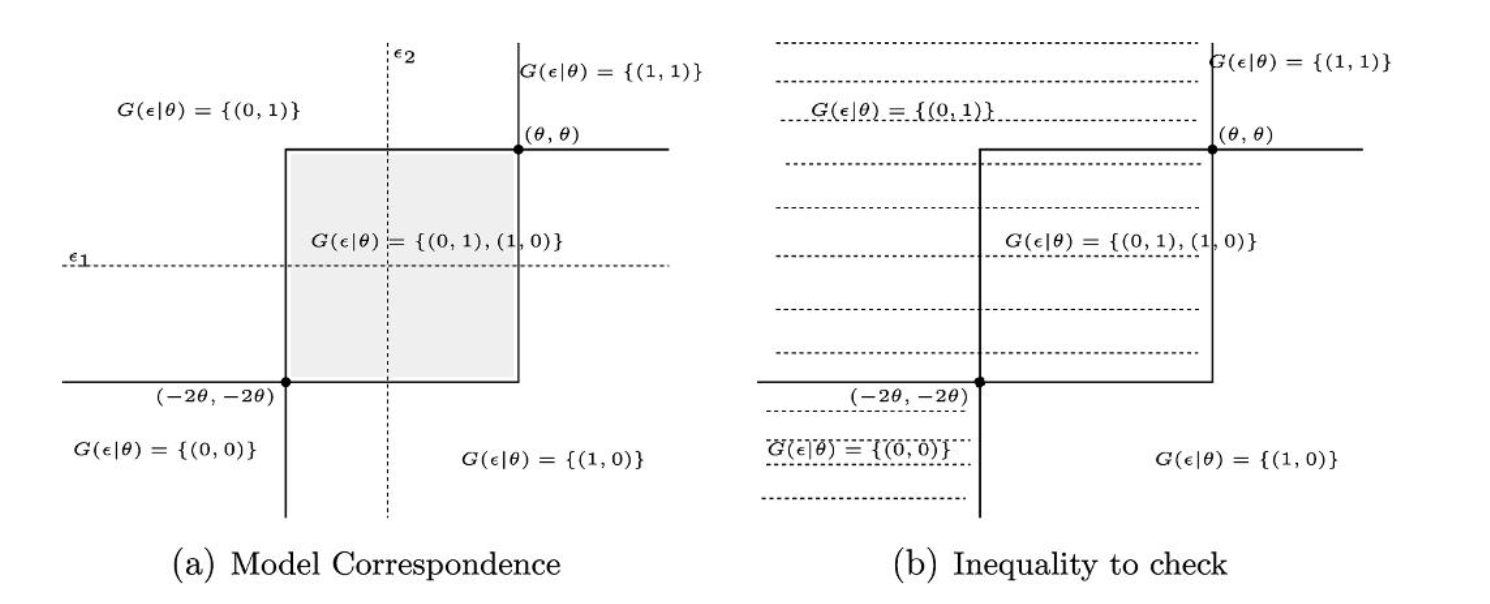
\includegraphics[width=0.95\textwidth]{figures/GH-Fig1}
	\caption{Family Game [Lifted from Paper]}
	\label{fig:GH-1}
\end{figure}

In the case of the family bargaining game, the set of possible outcomes is $\calY = \{(0,0),(0,1),(1,0),(1,1)\}$. The generalized likelihood of outcomes predicted by the model can be written as follows: 
\begin{align*}
 	\calL(\{(0,0)\}|\theta) &= \nu(\eps: \eps_1 \leq -2\theta, \eps_2 \leq -2\theta| \theta) = \nu(G^{-1}((0,0)|\theta)|\theta)\\
 	\calL(\{(0,1)\}|\theta) &= \nu(\eps: \eps_1 \leq \theta, \eps_2 \geq -2\theta| \theta) = \nu(G^{-1}((0,1)|\theta)|\theta)\\
 	\calL(\{(1,0)\}|\theta) &= \nu(\eps: \eps_1 \geq -2\theta, \eps_2 \leq \theta| \theta) = \nu(G^{-1}((1,0)|\theta)|\theta)\\
 	\calL(\{(1,1)\}|\theta) &= \nu(\eps: \eps_1 \geq \theta, \eps_2 \geq \theta| \theta) = \nu(G^{-1}((1,1)|\theta)|\theta)
\end{align*}
anf the generalized likelihood of the remaining events can be derived as follows 
\begin{align*}
	\calL(\{(0,0)\}\cup A | \theta) &= \calL(\{(0,0)\}|\theta) + \calL(A|\theta),\hbox{ }\text{ for all }A \subset \calY/\{(0,0)\}\\
	\calL(\{(1,1)\}\cup A | \theta) &= \calL(\{(1,1)\}|\theta) + \calL(A|\theta),\hbox{ }\text{ for all }A \subset \calY/\{(1,1)\} \\
	\calL(\{(0,1),(1,0)\}|\theta) &= 1 - \calL(\{(0,0),(1,1)\}|\theta)
\end{align*}
The generalized likelihood predicted by the model is the set function $A\mapsto \calL(A|\theta) = \nu(G^{-1}(A|\theta)|\theta)$ for $A \subset \calY = \{(0,0),(0,1),(1,0),(1,1)\}$. This set function is a Choquet capacity and if the support of $\nu$ is suffeciently large, the generalized likelihood sums to more than one because the region of multiple equilibria is ``counted twice''. 

Model is completed by adding an equilibrium selection mechanism that will pick out a single equilibrium for each value of the latent variable $\epsilon$ in the region of multiplicity. As formally defined previously, an equilibrium selection mechanism is a conditional probability $\pi(\cdot | \eps, X,\theta)$ with support included in $G(\eps|X;\theta)$. It is compatible with the data if the probabilities it predicts are equal to the true probablities of the observable variables. 

In this example, for $j = 0,1$:
\[P((i,j)|X) = \int_\calU \pi((i,j)|\eps, X;\theta)\nu(d\eps|X;\theta)\]
Since the model contains no prior information, any valid probability measure equilibrium selection mechanism that generates equates predicted probabilities with observed probabilities is consistent.

It is noted that the definition of the identified region using a semi-parametric likelihood representation, with the equilibrium selection mechanism as the infinite dimensional nuisance parameter $\pi$ is impractivle, so Theorem \ref{thm:GH-1} is used to make it operational and compute $\Theta_I$. So 
\[\Theta_I = \{\theta \in \Theta: (\forall A \in 2^\calY; P(A|X) \leq \calL(A|X;\theta); X-a.s\}\]

\subsection{Effecient Computation of the Identified Set}

Subtitle: ``\emph{Which inequalities to check and how to check them?}''

Describe three approaches to the effective computation of the identified set based on the characterization of Theorem~$\ref{thm:GH-1}$. First approach is based on submodular optimization and extends readily to the case with mixed strategies. Second appraoch, describes in Section 2.2, relies on the highly effecient algorithms for optimal transportation problems.\footnote{I found the following ArXiv introduction to optimal transport problems \href{https://arxiv.org/abs/1009.3856}{here} (if the link doesn't work; https://arxiv.org/abs/1009.3856)} Third approach is based off the notion of \emph{core determining sets} and provides a dramatic reduction in the computational complexity under specific assumptions on the game under study.

\subsubsection{Submodular Optimization}

The first proposal to deal with the complexity of the problem of checking inequalities in Theorem~\ref{thm:GH-1} is a method of general validity based on the minimization of a submodular function, the discrete equivalent of a convex function. This is a well-known problem in combinatorial optimiazation and effecient algorithms are easily available off the shelf. 

\begin{definition}[Submodular function]
	\label{def:GH-6}
	A set function $\calL:\calY\rightarrow\SR$ is called submodular if, for each $A, B \subset \calY$, we have 
	\[\calL(A\cup B) + \calL(A\cap B) \leq \calL(A) + \calL(B)\]
	In the case that $\calL$ is a probability measure, this holds as equality.
\end{definition}

Submodularity for set functions is the analogue of convexity, and the problem of minimizing a submodular function is well studied. Paper now shows that checking inequalities involved in the characterization of the identified set in Theorem~\ref{thm:GH-1} is equivalent to the minimization of a submodular function. Theorem~\ref{thm:GH-1} whoes that the identified set is the set of values of $\theta$ such that $X$-almost surely, we have the domination $\forall A\subseteq \calY$, $P(A|X) \leq \calL(A|X;\theta)$. Equivalently, 
\[\min_{A\subseteq\calY}\left(\calL(A|X;\theta) - P(A|X) \right) \geq 0\]
First note that the function above is indeed submodular.
\begin{lemma}[Submodularity of the generalized likelihood]
 	\label{lemma:GH-1}
	For all $\theta \in \Theta$ and all $X$, the set function $\calY$ defined for all $A\subseteq\calY$ by $A\mapsto \calL(A|X;\theta) - P(A|X)$ is submodular. 
\end{lemma}
 The most effecient, generic, way to check that a convex function is everywhere non-negative and verify that the minimum is non-negative. Apply the same logic to the above. Of course, can speed this up by terminating the algorithm when a negative value is found.

 \begin{theorem}[Computation of the identified set]
	\label{thm:GH-2}
	The identified set is obtained by minimization of a submodular function
	\[\theta_I = \left\{\theta \in \Theta: \min_{B\subseteq\calY} \left(\calL(B|X;\theta - P(B|X)\right)= 0, X-\text{a.s}\right\}\] 	
 \end{theorem}

As a note: I think the reason there is an ``$=0$'' instead of a $\geq 0$ in the statement of the identified set above is that we can always take $B=\emptyset$. More details on the procedure are given later on in Section 4. This method can be generalized to the case where equilibria in mixed strategies are considered.

The below is a special case of submodular optimization which is more effecient and applies to the case where only equilibria in pure strategies are considered.

\subsubsection{Optimal Transportation Approach}

When equilibria are only in pure strategies, the model generalized likelihood $\calL$ is a very special case of submodular function since it is derived as the distribution function of a random set. 
\[\calL(A|X;\theta) = \nu(\epsilon: G(\epsilon | X;\theta) \cap A \neq \emptyset| X;\theta)\]

When mixed equilibria are considered, this improvment in effeciency is no longer available because (in general), the model generalized likelihood is no longer the distribution of a random set.\footnote{Why not? Maybe because the probabilities of observing an outcome now are not functions of the underlying probability space $(\Omega, \calF, \mathbb{P})$, but, rather also depend on the properties of the mixed strategy equilibrium} To describe the method, need the following notations and definitions. 

Call $\calU^*$ the set of predicted combinations of equilibrium, formally $\calU^* = \{G(\epsilon|X;\theta); \epsilon \in \calU\}$, remembering that $\calU$ is the support of $\eps$. Note that $\calU^*$ is a quotient space for the correspondence $G$
\footnote{From WolframMathWorld: A quotient space, $X$/{\raise.17ex\hbox{$\scriptstyle\mathtt{\sim}$}} of a topological space $X$ and a set of equivalence classes {\raise.17ex\hbox{$\scriptstyle\mathtt{\sim}$}} on $X$ is the set of equivalence classes of points in $X$ (under {\raise.17ex\hbox{$\scriptstyle\mathtt{\sim}$}}). Open sets on $X$/{\raise.17ex\hbox{$\scriptstyle\mathtt{\sim}$}} can be described using the map $\pi: X\rightarrow X$/{\raise.17ex\hbox{$\scriptstyle\mathtt{\sim}$}} which maps each point in $X$ to its equivalence class. A subset $W \subseteq X$/{\raise.17ex\hbox{$\scriptstyle\mathtt{\sim}$}} is open if $\pi^{-1}(W)$ is open. $\calU^*$ is a quotient space for $\calU$ using equivalence classes from the correspondence $G$, that is $\calU = X/${\raise.17ex\hbox{$\scriptstyle\mathtt{\overset{G}\sim}$}} where $\eps_1{\raise.17ex\hbox{$\scriptstyle\mathtt{\overset{G}\sim}$}} \eps_2$ if $G(\eps_1) = G(\eps_2)$}. 
So $\calU^*$ contains subsets of $\calY$ but is typically of much lower cardinality than $2^\calY$. 

Further, consider the bipartite graph $\calG(\theta, X)$ in $\calY \times \calU^*$. The edges are defined as $(y,u) \in E(\calG)$ if $y \in u$. Each vertex $u \in \calY$ has weight $P(y|X)$ and each vertex $y\in \calU^*$ has weight $\nu(\{\epsilon: G(\epsilon|X;\theta) = u|X\})$. Finally, call $Q(\cdot|X;\theta)$ the probabilities $Q(u|X;\theta) = \nu\{G^{-1}(u)| X;\theta)\}$ (so t at $Q(u|X;\theta)$ is the weight attached to vertex $u \in \calY$.)

Theorem~\ref{thm:GH-1} shows that $\theta \in \Theta_I$ if and only if, for any subset $A$ of $\calY$, we have $P(A|X) \leq Q(G^{-1}(A)|X;\theta)$, where $G^{-1}(A) = \{u\in\calU^* | A\cap u \neq \theta\}$. Galichon and Genry show that it is equivalent to the existance of a joint probability $\Lambda$ on $\calG(\theta, X)$ with marginal distributions $P(\cdot| X)$ and $Q(\cdot|X;\theta)$.\footnote{I'm a bit lost on this part. I don't quite know what a probability is on a bipartite graph. I guess we just mean a joint probability distribution on the product space of the outcomes and the sets of outcomes. The theorem makes more sense intuitively looking at it from this view. For a consistent parameter, the rules relating the weights on one side with weights on the other are given above.}

\begin{theorem}
	\label{thm:GH-3}
	The parameter value $\theta$ belongs to the identified set iff there exists a probability on $\calY \times \calU^*$ with support contained in $G(X;\theta)$ and with marginal probabilities $P(\cdot|X)$ and $Q(\cdot|X;\theta)$. 
\end{theorem}

One implication is easy to prove. Call $U$ the random element with distribution $Q$ ($U$ is a random variable from $(\Omega, \calF, \mathbb{P}) \rightarrow \calY$) If a joint probability $\Lambda$ exists with all the required properties then 
\[Y\in A \implies U\in G^{-1}(A)\]
(Family Bargaining Example cont.) For the case of the family bargaining game 
\[\calU^* = \bigg\{\{(0,0)\}, \{(0,1)\}, \{(1,0)\}, \{(1,1)\}, \{(0,1),(1,0)\}\bigg\}\] 
This is a class of sets because $G(\eps|X;\theta)$ is a correspondence. The existence of a joint probability measure on $\calY \times \calU^*$ supported on $\calG(X;\theta)$ with marginal probabilities $p_y, y\in\calY$ and $q_u, u\in\calU^*$ can be represented graphically by a set of non-negative numbers attached to each edge of the graph that sum to 1, and such that the weight of each vertex is qual to the sum of the weights on the edges that reach it.


%!TEX root = /Users/manunavjeevan/Documents/GitHub/mnavjeev.github.io/files/Moment Inequality Methods/Annotated Literature Review/inequalityLitReview.tex

\newpage
\section{A Geometric Approach to Inference in Set-Identified Entry Games; \textit{\small Christian Bontemps, Rohit Kumar (JoE, 2020)}}\label{sec:BK-2020}

\citet{BK-2020} is set to appear in Journal of Econometrics in 2020. They consider inference procedures for entry games with complete information. Complete the model with the unknown selection mechanism and characterize geometrically the set of predicted choice probabilities. A 2019 version of the paper can be found 
\href{https://www.cemmap.ac.uk/uploads/Bontemps-Kumar-JofEc-december2019.pdf}{here}.

\subsection{Introduction}

Paper provides an estimation procedure for empirical models of entry and market structure. Entry games are popular in the empirical Industrial Organization literatures because they allow researchers to study the nature of firms' profits and the nature of competition between firms from data that are generally easy to collect. Popularized by the seminal works of Bresnahan and Reiss (1991a). 

Econometrics analysis of entry games is complicated by the presence of multiple equilibria, a problem that affects the standard estimation strategy.  Without additional assumptions, the model is incomplete. 

This paper completes the model with the selection mechanism $\eta(\cdot)$ and characterizes the set of predicted choice probabilities generated by the variation of $\eta(\cdot)$ in the space of admissible selection mechanisms. First contributions is to characterize more deeply the geometric structure of this set. 

Set ends up being a convex polytope with many facets (because of focus on pure strategy equilibrium). This paper derived a closed form expression for the support function of this polytope, the extreme points (or \emph{vertices}) of which can also be calculated as a function of the primitives of the model. Vertices are characterized by an order of outcome selection in the regions of multiple equilibria. Each vertex is also geometrically defined by the intersection of some supporting hyperplanes. Able to define the cone of outer normal vectors of these hyperplanes, and, thereby, the inequalities that are binding in this point.

Testing whether a parameter belongs to the identified set is equivalent to testing whether the true choice probability vector belongs to this convex set. However, when the number of players increases, the number of facets of the polytope increases exponentially, and, therefore, the smallest number of inequalities necessary to have a sharp characterization of the the identified set - from 16 in a game with 3 players to more than 1 million in a game with 6 players.

\subsection{Entry Game with \emph{N} players}

Formalize the entry game considered with $N$ firms. First consider a model without explanatory variables.

\subsubsection{Setup and Notations}

\paragraph{Model}
Let $N$ denote the number of firms that can enter any market. Following Berry (1992), introduce a model of market structure where the profit function $\pi_{im}$ of firm $i$ in a market $m$ is assumed to be independent of the identity of the firm's competitors. All firms decide simultaneously whether to enter the market (action \(a_{im} = 1\), doing so if their profit is positive. If $\pi_{im} = 0$, firms do not enter the market (take action \(a_{im}= 0\)). The profit function is assumed, without loss of generality, to be linear in the explanatory variables\footnote{[FOOTNOTE FROM TEXT] Any separable parametric form $\pi_{im} = f_i(\sum_{j\neq i} a_{jm}l\alpha) + \eps_{im}$ can be considered as long as the function $f_i(\cdot;\theta)$ is strictly decreasing in its first argument.}
\begin{equation}
	\label{eq:BK-1}
	\begin{split}
    	\pi_{im} &= \beta_i + \alpha_i \left(\sum_{j\neq i}a_{jm}\right) + \eps_{im} \\
    	a_{im} &= \ind\{\pi_{im} > 0\}
	\end{split}
\end{equation}


Following the literature, assume that $\alpha_i < 0$, i.e, the presence of more competitors decreases a firm's profit. Unobserved components $\eps_{im}, i = 1,\dots, N$ are drawn from a known distribution (up to some parameter vector $\gamma$). Econometrician does not observe their values but firms do.

For identification, we first need a scale normalization, and thus, assume that the variance of each shock $\eps_{im}$ is equal to 1. Denote the distribution of $\eps_m = (\eps_{1m},\dots, \eps_{Nm})^T$ and assume that the distribution is continuous with full support. Use notation $\theta$ for all the parameters in the model, and omit the subscript $m$ for notational convenience. Assume $\theta \in \Theta \subseteq \SR^l$. 

\paragraph{Multiplicity of Pure Strategy eqm.}

For a given market, an outcome $y$ is the vector of actions (in $\{0,1\}^N$) taken by the firms. There are $2^N$ possible outcomes. Denote by $\calY$ this set of possible outcomes. $\calY_K$ denotes the subset of outcomes with $K$ active firms in equilibrium, i.e any firms playing action 1. There is 1 outcome with 0 active firms, $N$ outcomes  with 1 active firm, $d_k = \binom{N}{K}$ with $K$ active firms, etc. 

Globally, order the outcomes in $\calY$ first by their number of active firms, then according to the predefined order within each $\calY_K$:
\[\calY = \left\{\underbrace{y_1^{(0)}\vphantom{,\dots,y_{d_K}^{(N)}}}_{\calY_0}, \underbrace{y_1^{(1)}, \dots, y_{d_1}^{(1)}}_{\calY_1}, \dots, \underbrace{y_1^{(K)},\dots,y_{d_K}^{(K)}}_{\calY_K},\dots, \underbrace{\vphantom{,\dots,y_{d_K}^{(N)}}y_1^{(N)}}_{\calY_N} \right\}\]

Well known that the model has multiple equilibria, regions of realizations of $\eps$ in which one cannot uniquely predict each firms' action. Consequently, no one-to-one mapping between the collection of possible outcomes and the regions of $\eps$ given any parameter value $\theta$. Consequently no one-to-one mapping between the collection of possible outcomes and the regions of $\eps$ given any parameter value $\theta$. 

Missing from the model is the selection of a given equilibrium in the regions of multiple equilibria. Define this selection mechanism $\eta(\cdot)$ as in Definition \ref{def:GH-2} of \citet{GH-2011}.

\begin{definition}[Equilibrium Selection Mechanism]
	\label{def:BK-1}
	An equilibrium selection mechanism is a conditional probability $\eta(\cdot | \eps; \theta)$ such that the selected value of the outcome variable is actually an equilibrium predicted by the game. That is $\supp(\eta(\cdot | \eps;\theta)) \subseteq G(\eps |\theta) $
\end{definition}

Denote by $\calE$ the set of selection mechanisms and by \(P(\theta,\eta)\) the predicted choice probability vector when the parameter of the model is is \(\theta\) and selection mechanism is $\eta(\cdot)$. Partition this vector according to the partition of $\calY$ as 
\begin{equation}
	\label{eq:BK-2}
	P(\theta,\eta) = \left(\underbrace{\vphantom{,\dots P_{d_k}^{(K)}(\theta,\eta)}P_1^{(0)}(\theta,\eta)}_{P^{(0)}(\theta,\eta)},\dots, \underbrace{P_1^{(K)}(\theta,\eta),\dots, P_{d_K}^{(K)}(\theta,\eta)}_{P^{(K)}(\theta,\eta)},\dots\underbrace{\vphantom{,\dots P_{d_k}^{(K)}}P_1^{(N)}(\theta,\eta)}_{P^{(N)}(\theta,\eta)}\right)^T
\end{equation}

One solution to the multiple equilibria problem consists of making assumption on this selection mechanism like in Reiss (1996) or Cleeren (2010). The vector of predicted choice probabilities is a point in $[0,1]^{2^N}$ and standard inference techniques may be used. Of course, any restrictions are ad hoc and may lead to misspecification. 

Another solution, following the literature on set-identification, consists of characterizing all the possible choice probabilities predicted by the model. The vector of predicted choice probabilities, instead of being an unrestricted point, belongs to a convex set that is characterized. Different sets of values $(\theta, \eta)$ may generate the same point $P(\theta,\eta)$. Goal is to characterize which ones generate the true (read: observed) choice probability vector. 

\subsubsection{Choice Probabilities to Identified Set}

Want to characterize the set of predicted choice probabilities. To do so, need to understand the multiplicity structure and characterize it. Then derive a parameterization of the set. 

\paragraph{Regions of Multiple Equilibria}

Specification ensures that multiple equilibria only involve outcomes with the same number of active firms, i.e within $\calY_K$. Therefore, focus on subsets of outcomes $S\subseteq \calY_K$ to characterize the multiple equilibria regions. Say that a subset $S\subseteq \calY_k$ is \textbf{in multiplicity} if the prediction of the game is all outcomes in $S$ and no outcome outside $S$ for $\eps$ in a non empty set $\calR_S^{(K)}(\theta)$.\footnote{In the Galichon Henry (2011) notation, this means that \(S = G(\eps|\theta)\) for some \(\eps \in \calU\). Then $\calR_S^{(K)}(\theta) = \{\eps \in \calU : G(\eps|\theta) = S\}$}
$\calR_S^{(K)}$ is called a multiple equilibria region. Denote by $S^{(K)}$ the collection of subsets $S$ of $\calY_K$ in multiplicity\footnote{The maximum number of such subsets is equal to $2^{d_K} - d_k - 1$}.
\[S^{(K)} = \left\{S\subset \calY_K: |S|\geq 2\text{ and $S$ is in multiplicity}\right\}\]
Note that not all subsets of cardinality greater than two are elements of $S^{(K)}$. For example, when $N = 4$, $K = 2$, $S_1 = \{(1,1,0,0)^T,(0,0,1,1)^T\}$ is not in multiplicity whereas the subset $S_2 = \{(1,1,0,0)^T,(1,0,1,0)^T\}$ is\footnote{This just means that, there exists a value of $(\theta,\eps)\in \Theta \times \SR^{N}$ such that both outcomes in $S_2$ are simultaneously equilibria of the game. That is, given $\theta$ and $\eps$, both $(1,1,0,0)^T$ and $(1,0,1,0)^T$ are equilibria. However, there is no value of $(\theta,\eps)$ such that both $(1,1,0,0)^T$ and $(0,0,1,1)^T$ are both simultaneously equilibrium outcomes.}.

Now present necessary and sufficient condition for $S$ to be in multiplicity. 
\begin{align*}
	N_0(S) &= \{\text{Set of indices of firms that always play action 0 across $S$}\} \\
	N_1(S) &= \{\text{Set of indices of firms that always play action 1 across $S$}\} 
\end{align*}
Further define $n_0(S) = |N_0(S)|$ and $n_1(S) = |N_1(S)|$, the cardinalities of the sets above. For now, suppress the dependence on $S$. With $N_0$ and $N_1$ fixed, there are $\binom{N - n_0 - n_1}{K - n_1}$ possible outcomes in $\calY_K$ corresponding to the remaining choice of the $K-n_1$ which play action $a_{im} = 1$ among the $N- n_0 - n_1$ remaining ones. $S$ should contain all these possibilities to be in multiple equilibria. 
\begin{prop}
	\label{prop:BK-1}
	A set $S\subset \calY_K$ is in multiplicity if and only if \(|S| = \binom{N- n_0 - n_1}{K - n_1}\)
\end{prop}
For the particular examples above, $S_1$ is not in multiplicity because $n_0 = n_1 = 0$ and, consequently, the subset should contain $\binom{4}{2} = 6$ outcomes with two active firms to be in multiplicity. $S_2$ is in multiplicity because $n_0 = n_1 = 1$ and it collects all possible outcomes, \(\binom{4-1-1}{2-1}=1\). Proof of proposition 1 also characterizes the region \(\calR_S^{(K)}(\theta)\).  Proposition \ref{prop:BK-1} can be used to count the number of multiple equilibria regions:
\begin{prop}
	\label{prop:BK-2}
	The cardinality of $S^{(K)}$, i.e, the number of multiple equilibria regions predicting $K$ active firms, for $1\leq K \leq N-1$ is equal to 
	\[|S^{(K)}| = \sum_{n_1 = 0}^{K-1} \sum_{n_0 = 0}^{N-K-1}\binom{N}{n_1}\binom{N-n_1}{n_0}\footnote{We can think of this as, for a given $K$ firms that are active in the quilibrium, choose $n_1$ to ``always'' be in and $n_0$ to ``always'' be out. So long as $n_0 + n_1 < N$ and $n_1 < K$, there is garunteed to be a region of mulitple equilibria corresponding to this by Proposition \ref{prop:BK-1}.}\]
\end{prop}
With $K=1$, the number of regions of multiple equilibria is $\sum_{n=0}^{N-2} \binom{N}{n}$, all possible combinations of more than two outcomes. However, Table \ref{table:BK-1} shows that the number of regions for the various values of $N$ and $K$ is generally far less than all the possible combinations. So the parameterization of the set of predicted choice probabilities is of a much lower dimension than one would have expected.
\begin{table}[htb!]
	\centering
	\begin{tabular}[c]{|lllll|}
		\hline\hline
		$N$ & $K$ & $d_k$ & $|S^{(K)}|$ & $2^{d_k} - d_k - 1$\\
		\hline
		3 & 1 & 3 & 4 & 4 \\ 
		  & 2 & 3 & 4 & 4 \\
		\hline 
		4 & 1 & 3 & 11 & 11 \\ 
		& 2 & 6 & 21 & 59 \\ 
		& 3 & 4 & 11 & 11 \\ 
		\hline 
		5 & 1 & 5 & 26 & 26 \\
		& 2 & 10 & 71 & 1018 \\
		& 3 & 10 & 71 & 1018 \\
		& 4 & 5 & 26 & 26 \\
		\hline 
		6 & 1 & 6 & 57 & 57 \\
		& 2 & 15 & 198 & 32761\\
		& 3 & 20 & 283 & 1048569 \\
		& 4 & 14 & 198 & 32761 \\ 
		& 5 & 6 & 57  & 57\\
		\hline\hline
	\end{tabular}
	\caption{Counting the number of multiple equilibria regions [Lifted from paper]}
	\label{table:BK-1}
\end{table}

\paragraph{The set of predicted choice probabilities} Also define the subset of $S^{(K)}$ that contains one specific outcome $y_j^\PK$ as 
\[S_j^\PK = \left\{S\in S^\PK : y_j^\PK \in S\right\}\]
Following \citet{BT-2007} and \citet{GH-2011}, can calculate the probability of observing outcome $y_j^\PK$. This probability depends on the parameter vector $\theta$ and the selection mechanism $\eta$. Specifically, letting $U_j^\PK(\theta)$ be the region in the support of $\eps$ which uniquely predicts the outcome $y_j^\PK$:
\begin{equation}
	\label{eq:BK-3}
	P_j^\PK(\theta,\eta) = \int_{U_j^\PK(\theta)} dF(\eps;\theta) + \sum_{S\in S_j^\PK} \int_{R_S^\PK(\theta)} \eta\left(y_j^\PK|\eps;\theta\right) dF(\eps;\theta)
\end{equation}
Denote by 
\[\Delta_j^\PK(\theta) :=\int_{U_j^\PK(\theta)} dF(\eps;\theta)\andbox \Delta_S^\PK(\theta) := \int_{R_S^\PK(\theta)} dF(\eps;\theta)\]
Let $A(\theta)$ be the set of $P(\theta;\eta)$ generated by the variation of $\eta$ in $\calE$\footnote{Recall \(\calE\) is the set of all valid equilibrium selection mechanisms.} and let $B_K^\theta$ be the set of $P^\PK(\theta, \eta)$ generated by the variation of $\eta$ in $\calE$, for $K = 0,\dots,N$. Formally
\[A(\theta):= \left\{P\in\SR^{2^N}: \exists \eta \in \calE, P = P(\theta,\eta)\right\} \andbox B_K(\theta) := \left\{P^\PK\in \SR^{d_K}: \exists \eta \in \calE, P^\PK = P^\PK(\theta, \eta) \right\}\]
Equation \ref{eq:BK-3} can then be viewed as a parameterization of the sets $A(\theta)$ and $B_K(\theta)$ where the ``parameters'' are the regions $\calR_S^\PK(\theta)$\footnote{This means that elements of the sets $A(\theta)$, $B_K(\theta)$ are characterized/fully determined by their corresponding regions $\calR$.}.

\paragraph{A characterization of the identified set} 

Let $P_0 = P(\theta_0,\eta_0)$ be the true choice probabilities generated by the ``true'' unknown parameter and selection mechanism. The identified set $\Theta_I$ is defined as the collection of points $\theta$ such that $P_0$ can be rationalized with a selection mechanism 
\begin{equation}
	\label{eq:BK-4}
	\Theta_I := \left\{\theta\in \Theta: \exists \eta\in\calE, P_0 = P(\theta,\eta) \right\}
\end{equation}
The following is easily verified and intuitive
\begin{equation}
	\label{eq:BK-5}
	\theta\in\Theta_I \iff P_0 \in A(\theta)
\end{equation}
So, can study $\Theta_I$ by studying the structure of $A(\theta)$. The following result holds:
\begin{prop}
	\label{prop:BK-3}
	\(A(\theta)\) is a convex subset of $\SR^{2^N}$, each $B_K(\theta)$ is a convex subset of $\SR^{d_K}$, and 
	\[A(\theta) = B_0(\theta) \times B_1(\theta)\times \dots \times B_N(\theta)\]
\end{prop}
The convexity of $A(\theta)$ is a general feature of an entry game and does not depend on this specification. The specific structure, the direct product nature, comes from the specification in Equation (\ref{eq:BK-1}). Structure simplifies some of the results to follow. 

Also, $B_K(\theta)$ is a point only when the number of active firms in equilibrium is $0$ or $N$, because there is no region of multiple equilibria involving these specific outcomes. Note that each $B_K(\theta)$ is strictly included in the cube, $\cube_K$, defined by 
\begin{equation}
	\label{eq:BK-6}
	\Delta_j^\PK(\theta) \leq P_j^\PK \leq \Delta_j^\PK(\theta) + \sum_{S\in S_j^\PK} \Delta_S^\PK(\theta), \forall j \in \{1,\dots, d_K\}
\end{equation}
This follows simply from the breakdown of $P_j^\PK$ in equation (\ref{eq:BK-3}), the following definitions of $\Delta_j^\PK$ and $\Delta_S^\PK(\theta)$, and that $0 \leq \eta(\cdot) \leq 1$.

$\Theta_I$, the identified set, is not convex, but it can be characterized by verifying that a point $P_0$ belongs to a convex set $A(\theta)$. Using Proposition \ref{prop:BK-3}, can decompose this condition to
\[P_0\in A(\theta)\iff \forall K \in \{0,1,\dots, N\}, P_0^\PK \in B_K(\theta)\]
\subsubsection{The Support Function and a First Selection of Moment Inequalities}

Following the convex literature, introduce the support function of each convex set $B_K(\theta)$. Tool has, in particular, been used in the set-identified literature, by Beresteanu and Molinari (2008) and Bontemps et al. (2012). Helps in generating the set of inequalities satisfied by $P_0$. First go over what a support function of a convex set is, and how it generates the inequalities that are the basis of inference procedure. The \emph{support function} of a convex set $A\subset \SR^d$ is defined as 
\[\delta^*(q;A)= \sup_{x\in A} q^T x\]
for all directions $q \in \SR^d$. This is depicted visually in Figure \ref{fig:BK-Fig1}, below. Generally, the domain of $\delta(\cdot)$ is restricted to $\mathbb{S}^{n-1}$
\begin{figure}[htb!]
	\centering
	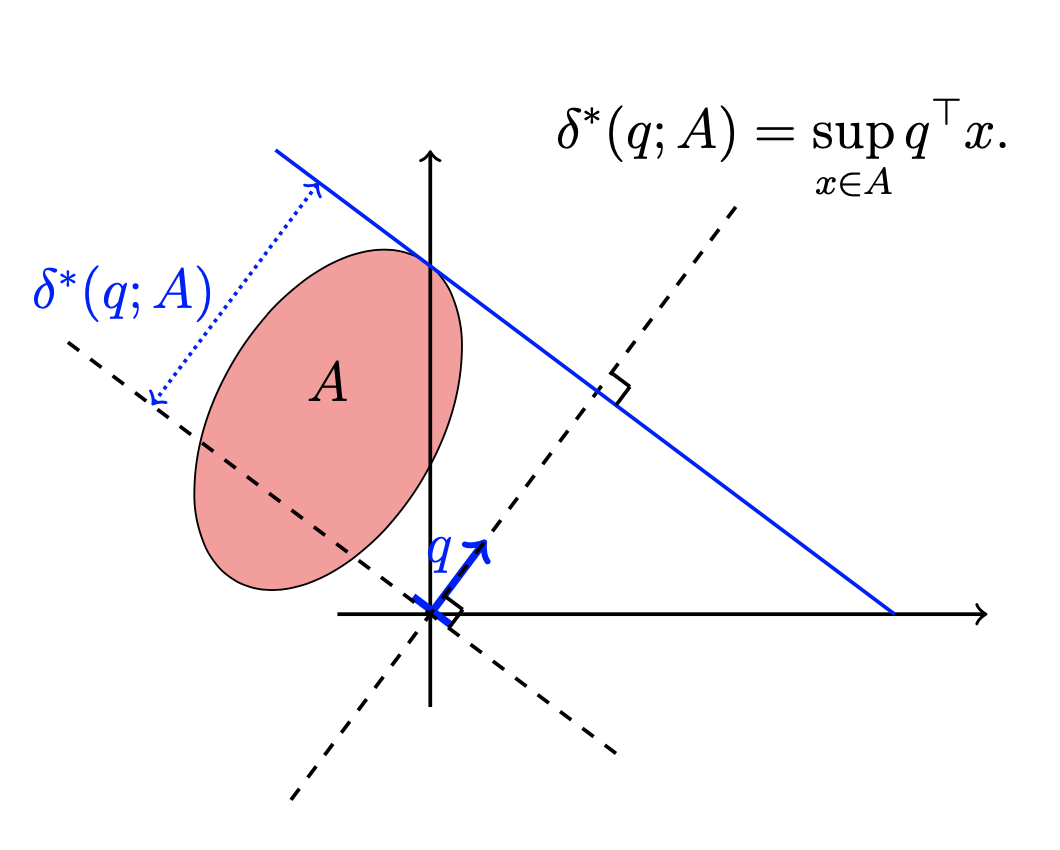
\includegraphics[width=0.50\textwidth]{figures/BK-Fig1.png}
	\caption{The support function [Lifted from \citet{BK-2020}]}
	\label{fig:BK-Fig1}
\end{figure}
The support function of a convex set in a given direction locates the supporting hyperplane in this direction. For each direction $q$, it defines an inequality that is satisfied by any point of the convex set. The support function implicitly gathers all the inequalities that define the convex set into a single function. If the set is smooth, there is a continuum of such inequalities. If it is a polytope, there are only a finite number of (linear) inequalities needed to characterize the set. \citet{KS-2014} show that, when the set is convex, using the support function leads to an efficient estimator of the convex identified set.

Following Rockafeller (1970) and Proposition \ref{prop:BK-3}, the identified set is characterized by the following inequalities.
\begin{equation}
	\label{eq:BK-7}
	\begin{split}
	 	\theta \in \Theta_I &\iff P_0 \in A(\theta) \\ 
	 	&\iff \forall q\in \SR^{2^N}, q^T P_0 \leq \delta^*(a;A(\theta)) \\
	 	&\iff \forall K, P_0^\PK \in B_K(\theta) \\
	 	&\iff \forall K, \forall q_K \in \SR^{d_K}, q_K^T P_0^\PK \leq \delta^*(q_K;B_K(\theta))
	 \end{split} 	
\end{equation} 
Breaking this down. $P_0$ is the observed ``true'' vector of outcome probabilities. \(A(\theta) \subset \SR^{2^N}\) is the set of probabilities that can be rationalized by an equilibrium selection mechanism in the model with parameter vector $\theta$. $P_0^\PK \in \SR^{d_K}$ is the sub-vector of probabilities for outcomes with $K$ active firms, where $d_K = \binom{N}{K}$, the number of possible outcomes with $K$ active firms. $B_K(\theta) \subset \SR^{d_K}$ is the set of sub-vectors of observed probabilities for outcomes with $K$ active firms that can be rationalized by an equilibrium selection mechanism in a model generated by parameter vector $\theta$.

Now turn to the calculation of the support function of $B_K(\theta)$ for any $K$. Make the following notations:
\begin{enumerate}
	\item  Let $q_K \in \SR^{d_K}$ be a given direction. Assume the following order among the coordinates of $q_K$: $q_{i_1,K} \geq q_{i_2,K} \geq \dots, \geq q_{i_{d_K},K}$. 
	\item Partition $S^\PK$, the collection of subsets of outcomes with $K$ active firms in multiplicity, as follows:  
	\begin{enumerate}
		\item Denote $\calO^\PK_{i_1} = S_{i_1}^\PK$\footnote{Remember $S_j^\PK = \{S \in S^\PK: y_j \in S\}$}, the elements of $S^\PK$ which contain the outcome $y_{i_1}^\PK$\footnote{$y_{i_1}^\PK$ being the outcome with $K$ active firms that has the highest probability assigned to it by $q_K \in \SR^{d_K}$}.
		\item Denote by $\calO^\PK_{i_2} \subset S_{i_2}^\PK$ the subset of elements of $S_{i_2}^\PK$ that are not in $\calO_{i_1}^\PK$, i.e $\calO_{i_2}^\PK = S_{i_2}^\PK \setminus S_{i_1}^\PK$.
		\item Continue on in this fashion for each $i_j, j \in 3, \dots, d_K$ defining 
		\[\calO_{i_j}^\PK = S_{i_j}^\PK \setminus \bigcup_{k < j} S_{i_k}^\PK\]
	\end{enumerate}
\end{enumerate}
Note that the construction of the outcomes $\calO_j^\PK$ is lined to the order of the components of $q_k$. Now provide a closed form expression for the support function in this direction (Prop \ref{prop:BK-4}, below).
\begin{prop}
	\label{prop:BK-4}
	Let $q_k\in\SR^{d_K}$ and assume $q_{i_1,K}\geq q_{i_2,K}\geq\dots,\geq q_{i_{d_K},K}$. The support function in the direction $q_K, \delta^*(q_k;B_K(\theta))$ is equal to 
	\begin{equation}
		\label{eq:BK-8}
		\delta^*(q_K;B_K(\theta)) = \sum_{j=1}^{d_K} q_{j,K}\Delta_j^\PK(\theta) + \sum_{j=1}^{d_K} q_{i_j,K}\left(\sum_{S\in\calO_{i_j}^\PK} \Delta_S^\PK (\theta)\right)
	\end{equation}
	it is reached at the extreme point 
	\begin{equation*}
		E_{i_1,i_2,\dots,i_{d_K}}^\PK = \vec\left(\Delta_1^\PK(\theta) + \sum_{s\in\calO_{1}^\PK} \Delta_S^\PK(\theta), \dots, \Delta_{d_K}^\PK(\t) + \sum_{S\in \calO_{d_K}}^\PK \Delta_S^\PK(\t) \right)
	\end{equation*}
	Consequently, $B_K(\theta)$ is a polytope and its vertices are included in the set of points $E_{i_1, i_2, \dots, i_{d_K}}^\PK$ where the vector if indices is any permutation of the vector of indices $(1,2,\dots, d_K)$. As such $B_K(\theta)$ has at most $d_K! = \binom{N}{K}!$ vertices.
\end{prop}

Each extreme point of $B_K(\t)$ can be calculated from the knowledge of the non-zero values of $\Delta_S^\PK(\theta), S \in S^\PK$. This number of non-zero values is the number of multiple equilibria refions, and we saw in Proposition \ref{prop:BK-2} that this number is much smaller than $2^{\binom{N}{K}} - \binom{N}{K} - 1$. Consequently, the parameterization of $B_K(\theta)$ is numerically tractable for moderate values of $N$. Furthermore, each non-zero value $\Delta_S^\PK(\t)$ can be easily calculated or simulated from the knowledge of the distribution of $\eps$. 

Can now extend this result to the calculation of the support function of the full set $A(\t)$ for any direction $q \in  \SR^{2^N}$. Adopt the standard notation $q = \vec(q_0, q_1, \dots, q_N)$ where $q_N$ is the direction related to the set $B_K(\t)$ (i.e $q_K \in \SR^{d_K}$) and $\vec(\cdot)$ denotes vertical concatenation. 

\begin{prop}
	\label{prop:BK-5}
	The support function of $A(\t)$ in the direction $q$ is equal to 
	\begin{equation}
		\label{eq:BK-9}
		\delta^*(q;A(\theta)) = \sum_{k=0}^N \delta^*(q_k;B_K(\t))
	\end{equation}
\end{prop}

Results come from the specific characterization of $A(\theta)$ in proposition $3$. The last proposition, combined with equation~\eqref{eq:BK-7}, is the basis of the inference problem. It generates a continuum of inequalities that have to be satisfied for any parameter of the identified set. However, since all the $B_K(\t)$'s and therefore, $A(\t)$ are polytopes, it is necessary and sufficient to test the inequalities in a finite set of directions. Now explicit this set of directions, first for the $B_K(\t)$'s and then for $A(\theta)$. Let $\calQ_K$ be the set of non-null directions of $\SR^{d_K}$ with coordinates that are either one or zero. There are $2^{d_K} - 1$ elements in $\calQ_K$. The next proposition shows that is sufficient to check the inequalities in $\calQ_K$, fo all $K$, to characterize the identified set:
\begin{prop}
	\label{prop:BK-6}
	Let $P_0\in\SR^{2^N}$ denote the observed vector of probabilities. Then
	\[\theta\in\T_I \iff \forall K \in \{0,1,2,\dots, N\}, \forall q_K \in \calQ_K, q_K^T P_0^\PK \leq \delta^*(q_K;B_K(\t))\]
\end{prop}
\textbf{Remark} Already mentioned that the specification ensures that the number of firms entering the market is constant among outcomes in multiplicity. As a result, the sets $B_K(\t)$ belong to a hyperplane because the sum of the components of $P^\PK(\t,\eta)$ is a constant which depends on $\t$ only. If we wanted to characterize one $B_K(\t)$ only, for one specific choice of $K$, would need to consider all the directions of $\calQ_K$ combined with the direction $(-1,-1,\dots, -1)$ to ensure the equality of the sum of all components. Here, due to the fact that we are considering. 

\paragraph{Optimal Transport, Random Sets, or Completion of the Model} Approach consists in characterizing the set $A(\theta)$ through its support function and extreme points. This is done after having completed the model with the unknown selection mechanism $\eta(\cdot)$ and finding which selection mechanisms generate the extreme points. Geometric structure induced by the multiplicities allows us to exhibit the inequalities that are satisfied by any parameter of the identified set. 

\citet{GH-2011} use optimal transportation theory and the notion of core determining classes to generate the relevant inequalities that characterize sharply the identified set. \citet{BMM-2011} emphasize that an entry game is a model with convex predictions. They use random set theory, and, in particular, the Aumann expectation considered in their paper is the set $A(\t)$. Both methods are numerically challenging for a game with 6 players even when considering only pure strategy equilibria. Following Proposition~\ref{prop:BK-6} there are, at maximum $\sum_{K=0}^N (2^{d_K} - 1)$ inequalities. However, this number is very large when $N\geq 6$; have more than 1 million inequalities to check. \citet{CT-2009} bound the sets $B_K(\t)$ by the cubes $Cub_K$, introduced above, which are easier to characterize. Their approach can handle games with a moderate number of players above 6, but sharpness is not attained. 

Fundamentally, whether one uses random set theory and the capacity functional, the optimal transport approach of \citet{GH-2011} or the approach presented in this paper, all methods are intended to derive a sufficient set of inequalities satisfied by the parameters in a specific manner. Each method has its specificities. However, this approach allows us to go deeper into the geometric analysis of the set $A(\t)$ and this is the objective of the next section. 

\subsection{Using the Geometry of \texorpdfstring{$A(\t)$}{} to Select Inequalities}

The convex set $B_K(\t)$ can be characterized by at most $2^{d_K} - 1$ inequalities. Due to its particular geometry, it may be the case that some of these inequalities. In this section, present two strategies to reduce the number of inequalities. The first consists of calculating a core determining class introduced by \citet{GH-2011} and later used in \citet{CR-2017}. Second consists of exploiting the geometry to propose a geometric selection procedure of the inequalities without having to evaluate all of them. 

\subsubsection{Deriving a Core Determining Class of an Entry Game}

Core determining classes yields a collection of non-redundant moment inequalities that are sufficient to sharply characterize the identified set $\T_I$. Provide a characterization of the core determining class in an entry game from the geometric study of the multiplicity structure of the model. 

As a reminder, 
\begin{definition}[Choquet Capacity]
	\label{def:BK-2}
	$\calL: 2^\calY \to \SR$ is a \emph{Choquet Capacity} if it is 
	\begin{enumerate}
		\item \emph{normalized}: $\calL(\emptyset) = 0$ and $\calL(\calY) = 1$, and 
		\item \emph{monotone}: $\calL(C) \leq \calL(B)$, for any $C\subseteq B\subseteq \calY$
	\end{enumerate}
\end{definition}

\begin{definition}[Core Determining]
	\label{def:BK-3}
	$\Omega \subset 2^\calY$ is called core determining for the Choquet Capacity $\calL$ on $\calY$ if, for an arbitrary random variable $X$ taking values on $\calY$ and associated law $\P$ (arbitrary probability distribution $\P$ on $\calY$):
	\[\P(C) \leq \calL(C), \forall C\in\Omega \implies \P(C) \leq \calL(C), \forall C \in 2^\calY\]
\end{definition}

The set $A(\t)$ is characterized by its support function. Thus, define the Choquet Capacity for a subset $C_K \subseteq \calY_K$ as
\begin{equation}
	\label{eq:BK-10}
 	\calL(C_K) = \delta^*(e_{C_K}; B_K(\theta)) = \max_{\eta\in\calE}\left(\sum_{j|y_j^\PK \in C_K} P_j(\t,\eta)\right)
 \end{equation} 
where $e_{c_K} \in \{0,1\}^{d_K}$ with $(e_{c_K})_j = 1$ if $y_j^\PK \in C_K$ and 0 otherwise. For a collection of subsets $C = \{C_K \subset \calY_K: K \leq N\}$, the Choquet capacity is defined as $\calL(C) = \sum_{k=0}^N \calL(C_K)$. $\calL$ is monotone, as it is the sum of quantities that are positive, and $\calL(\calY) = 1$. 

Define the concept of connectedness, which is useful for the exposition, introduced by \citet{GH-2011}. For a subset $C_K \subset \calY_K$, define the (undirected) graph generated by $C_K$ as $\Gamma_{C_K} = (C_K, E)$. For any graph $\Gamma = (V, E)$, we say that $C \subseteq V$ is \textbf{connected in the graph} $\Gamma$ if there is a path of elements of $E$ connecting any pair of nodes of $C$. 

\begin{definition}[Well Connectedness]
	\label{def:BK-4}
	A subset $C_K \subseteq \calY_K$ is called well connected in $\calY_K$ if $\calY_K \setminus C_K$ is connected in the graph $\Gamma_{\calY_K\setminus C_K}$\footnote{This is the subgraph obtained by deleting all nodes in $C_k$ and all associated edges.}.
\end{definition}

Note that $\calY_K$ is in multiplicity. Therefore, the graph $\Gamma_{\calY_K}$ is connected, and every $C_K \subseteq \calY_K$ is connected in the graph $\Gamma_{\calY_K}$. The notion of well connectedness extends the notion of connectedness by imposing restrictions on the complement of $C_K$. 

The graph $\Gamma_\calY$ is not connected, as there is no multiplicity between $\calY_K$ and $\calY_{K'}$ for $K\neq K'$. The $\Gamma_{\calY_K}$ is a component of $\Gamma_\calY$\footnote{Components have no edges between them.} Collect all well-connected subsets of $\calY_K$ as 
\[\Omega_K = \{C_K \subseteq \calY_K : C_K\text{ is well connected in }\calY_K\}\]
\citet{GH-2011} present some models in which the core determining class can be of much lower cardinality than $2^{|\calY|}$ by exploiting the monotonicity property in certain submodular games. However, their approach does not provide a way to find a core determining class for a general entry game. \citet{CR-2017} provide a sufficient condition to characterize a core determining class of set-identified models that can be written into what they call a generalized IV model. Next proposition provides a complete characterization of a core determining class for entry model through a necessary and sufficient condition.
\begin{prop}
	\label{prop:BK-7}
	A collection $\Omega$ of subsets of $\calY$ ($\Omega \subseteq 2^\calY$) is core determining for $\calL$ as defined in equation~\eqref{eq:BK-10} if and only if $\Omega = \{\Omega_K: K = 0, 1, \dots, N\}$.
\end{prop}

This selection, however, does not significantly reduce the number of non-redundant moment inequalities in the entry game. For example, when $N = 6$ and $K = 3$, it eliminates fewer than $30,000$ inequalities from a total of $2^{20} - 1 = 1,048,575$. 

\subsubsection{A Geometric Selection Procedure}

The core determining class is a useful concept since it eliminates redundant inequalities. However, it does not significantly reduce the number of inequalities in the entry game. This section presents a geometric selection procedure that fully exploits the geometery of the sets $B_K(\t)$. Procedure first selects the extreme point of the set that seems closes to the vector $P_0^\PK$ and then only evaluates only the ineqaulities associated with this extreme point (i.e tests the directions that are the outer normal vector of the supporting hyperplans of $B_K(\t)$ at this point, for each $K = 0, \dots, N$)\footnote{By extreme point I believe the authors mean a point $x \in A(\t)$ at which the support function $\delta(P_0, A(\t))= x^T P_0$}.

Following Proposition $4$, an extreme point is determined by an order in the coordinates (note that, a priori, two different orders couldlead to the same physical point). The first part of the algortihm is intended to determine this order in a recursive manner by exploting the position of $P_0^\PK$ with respect to the cube $\cube_K$ which contains $B_K(\t)$. 

Explain the steps in non-technical detail here and then formalize in the appendix.

\textbf{Local Moment Selection:} The local moment selection procedure can be summarized as follows.
\begin{enumerate}
	\item Determine the cube $\cube_K$ that contains $B_K(\t)$ by calculating the minimum and maximum of each coordinate. Them, determine which coordinate of $P_0^\PK$ is the furthest fromt he center of the cube. 

	\item Assume this is the $j^{\text{\emph{th}}}$ coordinate.
	\begin{enumerate}
		\item If it is on the maximum side, the extreme point is of the type $E_{j,?, \dots, ?}^\PK(\t)$ and now have to determine the next component. To do so, project $P_0^\PK$ on the face and repeat the previous calculation by taking into account that we are on the face that maximizes the $j^{\text{\emph{th}}}$ coordinate.
		\item If it is on the minimum side, know that extreme point will be of the form $E_{?,\dots, ?, j}^\PK(\t)$. Now have to determine the next component. To do so, project $P_0^\PK$ on this face and repeat the previous calculation, taking into accound that we are on the face that minimizes the $j^{\text{\emph{th}}}$ coordinate. 
	\end{enumerate}
	\item Repeat the following steps until having found one order of coordinates. 
	\item Once the local extreme point $E_{i_1, i_2, \dots, i_{d_K}}^\PK$ is determined, can focus on the directions of the local supporting hyperplans. Let the $d_K$ directions $e_{i_1}, e_{i_1, i_2}, \dots, e_{{i_1}, {i_2}, \dots, i_{d_K}}$, where the components are equal to $1$ and indices are subscrips of $e$ and $0$ otherwise. This set of directions is included in the set of directions of the local supporting hyperplanes. Only checking these directions doens't provide a sharp characterization of $B_K(\t)$ unless $K= 1$ or $K = N-1$, but, however, provides an important refinement with respect to the existing method of \citet{CT-2009}.
\end{enumerate}

Procedure selects which moments among the $2^{d_K} - 1$ are potentially binding without having to evaluate all of them. Selection is based on the spatial location of the point $P^\PK$ and exploits the geometery of the set $B_K(\t)$

\begin{prop}
	\label{prop:BK-8} Our local moment selection procedure provides a sharp characterization of the identified set for $N=3$. 
\end{prop}

\subsection{Estimation and Inference}

Following the results derived, now adopt the approach developed in \citet{BM-2008} and \citet{BMM-2012} for testing a pointin a convex set.
\begin{align*}
	\t \in \T_I(\P) &\iff P_0\in A(\t)\\
					&\iff \forall q \in \calG, T_{\infty}(q;\theta) = \delta^*(q;A(\t)) - q^T P_0 \geq 0 \\
					&\iff \min_{q\in\calG} T_\infty(q;\t) \geq 0 
\end{align*}

where $P_0$ is the true (observed) choice probability. The set of directions $\calG$ is defined as 
\[\calG = \bigcup_{K=0}^N \left\{\vec\left(0_{\sum_{i=1}^{K-1} d_i}, q_k, 0_{\sum_{i=K+1}^N} d_i\right): q_K \in \calG_K\right\}\]
where, either $\calG_K = \calQ_K$ as defined in Proposition~\ref{prop:BK-6} or $\calG_K = \Omega_K$, the core determining class characterized in Proposition~\ref{prop:BK-7}. The set $\calG$ collects all the directions needed to sharply identify the identified set. 

Test based on $T_\infty(\cdot)$ is infeasible because $P_0$ is not observed. Now characterize the feasible test statistic and its asymptotic distribution. Throughout this section, assume observe a sample of $M$ i.i.d markets in which the same $N$ firms compete. 

\subsubsection{The Asymptotic Distribution of the Test Statistics}

Let $T_M(q;\theta)$ be the empirical counterpart of $T_\infty(q;\t)$: 
\[T_M(q;\theta) = \delta^*(q;A(\t)) - q^T\hat{P}_M\]
Want asymptotic results to be valud, not only for the true probability, but also uniformly in the neighborhood around the true probability. Impose the following uniform integrability condition:

\begin{assumption}
	\label{assm:BK-1}
	The class $\calP$ of probability distributions satisfies 
	\begin{equation}
		\label{eq:BK-UI}
		\lim_{\lambda\to\infty} \sup_{P\in \calP} \sup_{j\in\{1,\dots,2^N\}}\E_P\left[\left(\frac{\ind(Y = y_j) - \mu_j(P)}{\sqrt{\mu_j(P)(1-\mu_j(P))}}\right)^2\ind\left\{\left|\frac{\ind(Y = y_j) - \mu_j(P)}{\sqrt{\mu_j(P)(1-\mu_j(P))}}\right| > \lambda \right\}\right] = 0
	\end{equation}
	where $\mu_j(P) = \E_P(Y = y_j)$
\end{assumption}
Assumption~\ref{assm:BK-1} ensures the uniform convergence of test statistic over the class of probability distributions. This condition is satisified over the class of probability distributions such that $\mu_j(P) \geq \eps$ for each $j$ and some $\eps > 0$.

\textbf{NOTE:} Rest of this discussion seems to follow standard asymptotic theory with the number of inequalities being tested remaining fixed as $n\rightarrow\infty$. This seems like the wrong setting.

Interested in covering a specific point in the identified set with some pre specified probability 
\[\liminf_{M\to\infty} \inf_{P\in\calP}\inf_{\theta\in\Theta_I(P)} \P(\t\in\calC_M) \geq 1 - \alpha\]
Following \citet{BMM-2012}, inference method is based on $T_M(q;\t)$, rescaled by $\sqrt{M}$ and normalized. 
\[\xi_M(\t) = \sqrt{M} \min_{q\in\calG} \frac{T_M(q;\t)}{\sqrt{q^T \hat{\Sigma}_q}}\]
A point $\t$ belongs to the confidence interval if the test based on $\xi_M(\t)$ is not rejected. Now calculate the asymptotic distribution of the test statistics $\xi_M(\t)$ 
\begin{prop}
	\label{prop:BK-9}
	Let $Q_\t$ be the set of minimizers of $T_\infty(q;\t)$ in $\calG$. Let $Z$ be a random vector of $\SR^{2^N}$ distributed according to the normal distribution with variance $\Sigma_0$. We have 
	\begin{equation*}
		\begin{cases}
			\xi_M(\t) \wcov \min{q \in Q_\t} \frac{q^T Z}{\sqrt{q^T\Sigma q}} &\text{ if } P_0 \in A(\t)\\
			\xi_M(\t) \rightarrow_{\text{a.s}} -\infty &\text{ if }P_0\not\in A(\t)
		\end{cases}
	\end{equation*}
	Under Assumption~\ref{assm:BK-1}, these results are uniformly valid over $P\in\calP$.
\end{prop}
Asymptotic distribution only depends on $\t$ through $Q_\t$





























% Gap before references
\newpage

% Bibliography
\bibliography{references}

\end{document}



